\documentclass[usenames,dvipsnames]{beamer}
\usepackage[mode=buildnew]{standalone}

\mode<presentation> {

\usetheme{Madrid}

\setbeamertemplate{footline} % To remove the footer line in all slides uncomment this line
%\setbeamertemplate{footline}[page number] % To replace the footer line in all slides with a simple slide count uncomment this line

%\setbeamertemplate{navigation symbols}{} % To remove the navigation symbols from the bottom of all slides uncomment this line
}

\usepackage{graphicx} % Allows including images
\usepackage{booktabs} % Allows the use of \toprule, \midrule and \bottomrule in tables
\usepackage{amsmath, amsfonts, amsthm, mathrsfs,bm}
\usepackage{xcolor}
\usepackage{siunitx}
\usepackage{tikz}
\usetikzlibrary{matrix,backgrounds,calc,shapes,arrows,arrows.meta,fit,positioning}
\usetikzlibrary{chains,shapes.multipart}
\usetikzlibrary{shapes,calc}
\tikzset{cross/.style={cross out, draw=black, fill=none, minimum size=2*(#1-\pgflinewidth), inner sep=0pt, outer
sep=0pt}, cross/.default={2pt}}
\usepackage{pgfplots}
\usepackage{varwidth}
%\pgfplotsset{compat=1.13}

%----------------------------------------------------------------------------------------
%	TITLE PAGE
%----------------------------------------------------------------------------------------

% The short title appears at the bottom of every slide, the full title is only on the title page
\title[Short title]{HPC-based FE$^2$ method implementation for large scale composite material problems}

\author{G. Giuntoli, M. V\'azquez, S. Oller} % Your name
\institute[BSC-UPC] % Your institution as it will appear on the bottom of every slide, may be shorthand to save space
{
Barcelona Supercomputing Center\\Universitat Polit\`ecnica de Catalunya \\ % Your institution for the title page
\medskip
\textit{guido.giuntoli@bsc.es} % Your email address
}
\date{\today} % Date, can be changed to a custom date

\begin{document}

\begin{frame}
\titlepage % Print the title page as the first slide
\end{frame}

%\begin{frame}
%\frametitle{Overview} % Table of contents slide, comment this block out to remove it
%\tableofcontents % Throughout your presentation, if you choose to use \section{} and \subsection{} commands, these will automatically be printed on this slide as an overview of your presentation
%\end{frame}

%----------------------------------------------------------------------------------------
%	PRESENTATION SLIDES
%----------------------------------------------------------------------------------------

%------------------------------------------------
%\section{First Section} % Sections can be created in order to organize your presentation into discrete blocks, all sections and subsections are automatically printed in the table of contents as an overview of the talk
%------------------------------------------------

%\subsection{Subsection Example} % A subsection can be created just before a set of slides with a common theme to further break down your presentation into chunks

%------------------------------------------------

\begin{frame}
\frametitle{Problem to solve}
\begin{figure}[!ht]
\resizebox{0.4\linewidth}{!}{\documentclass{standalone}

\begin{document}

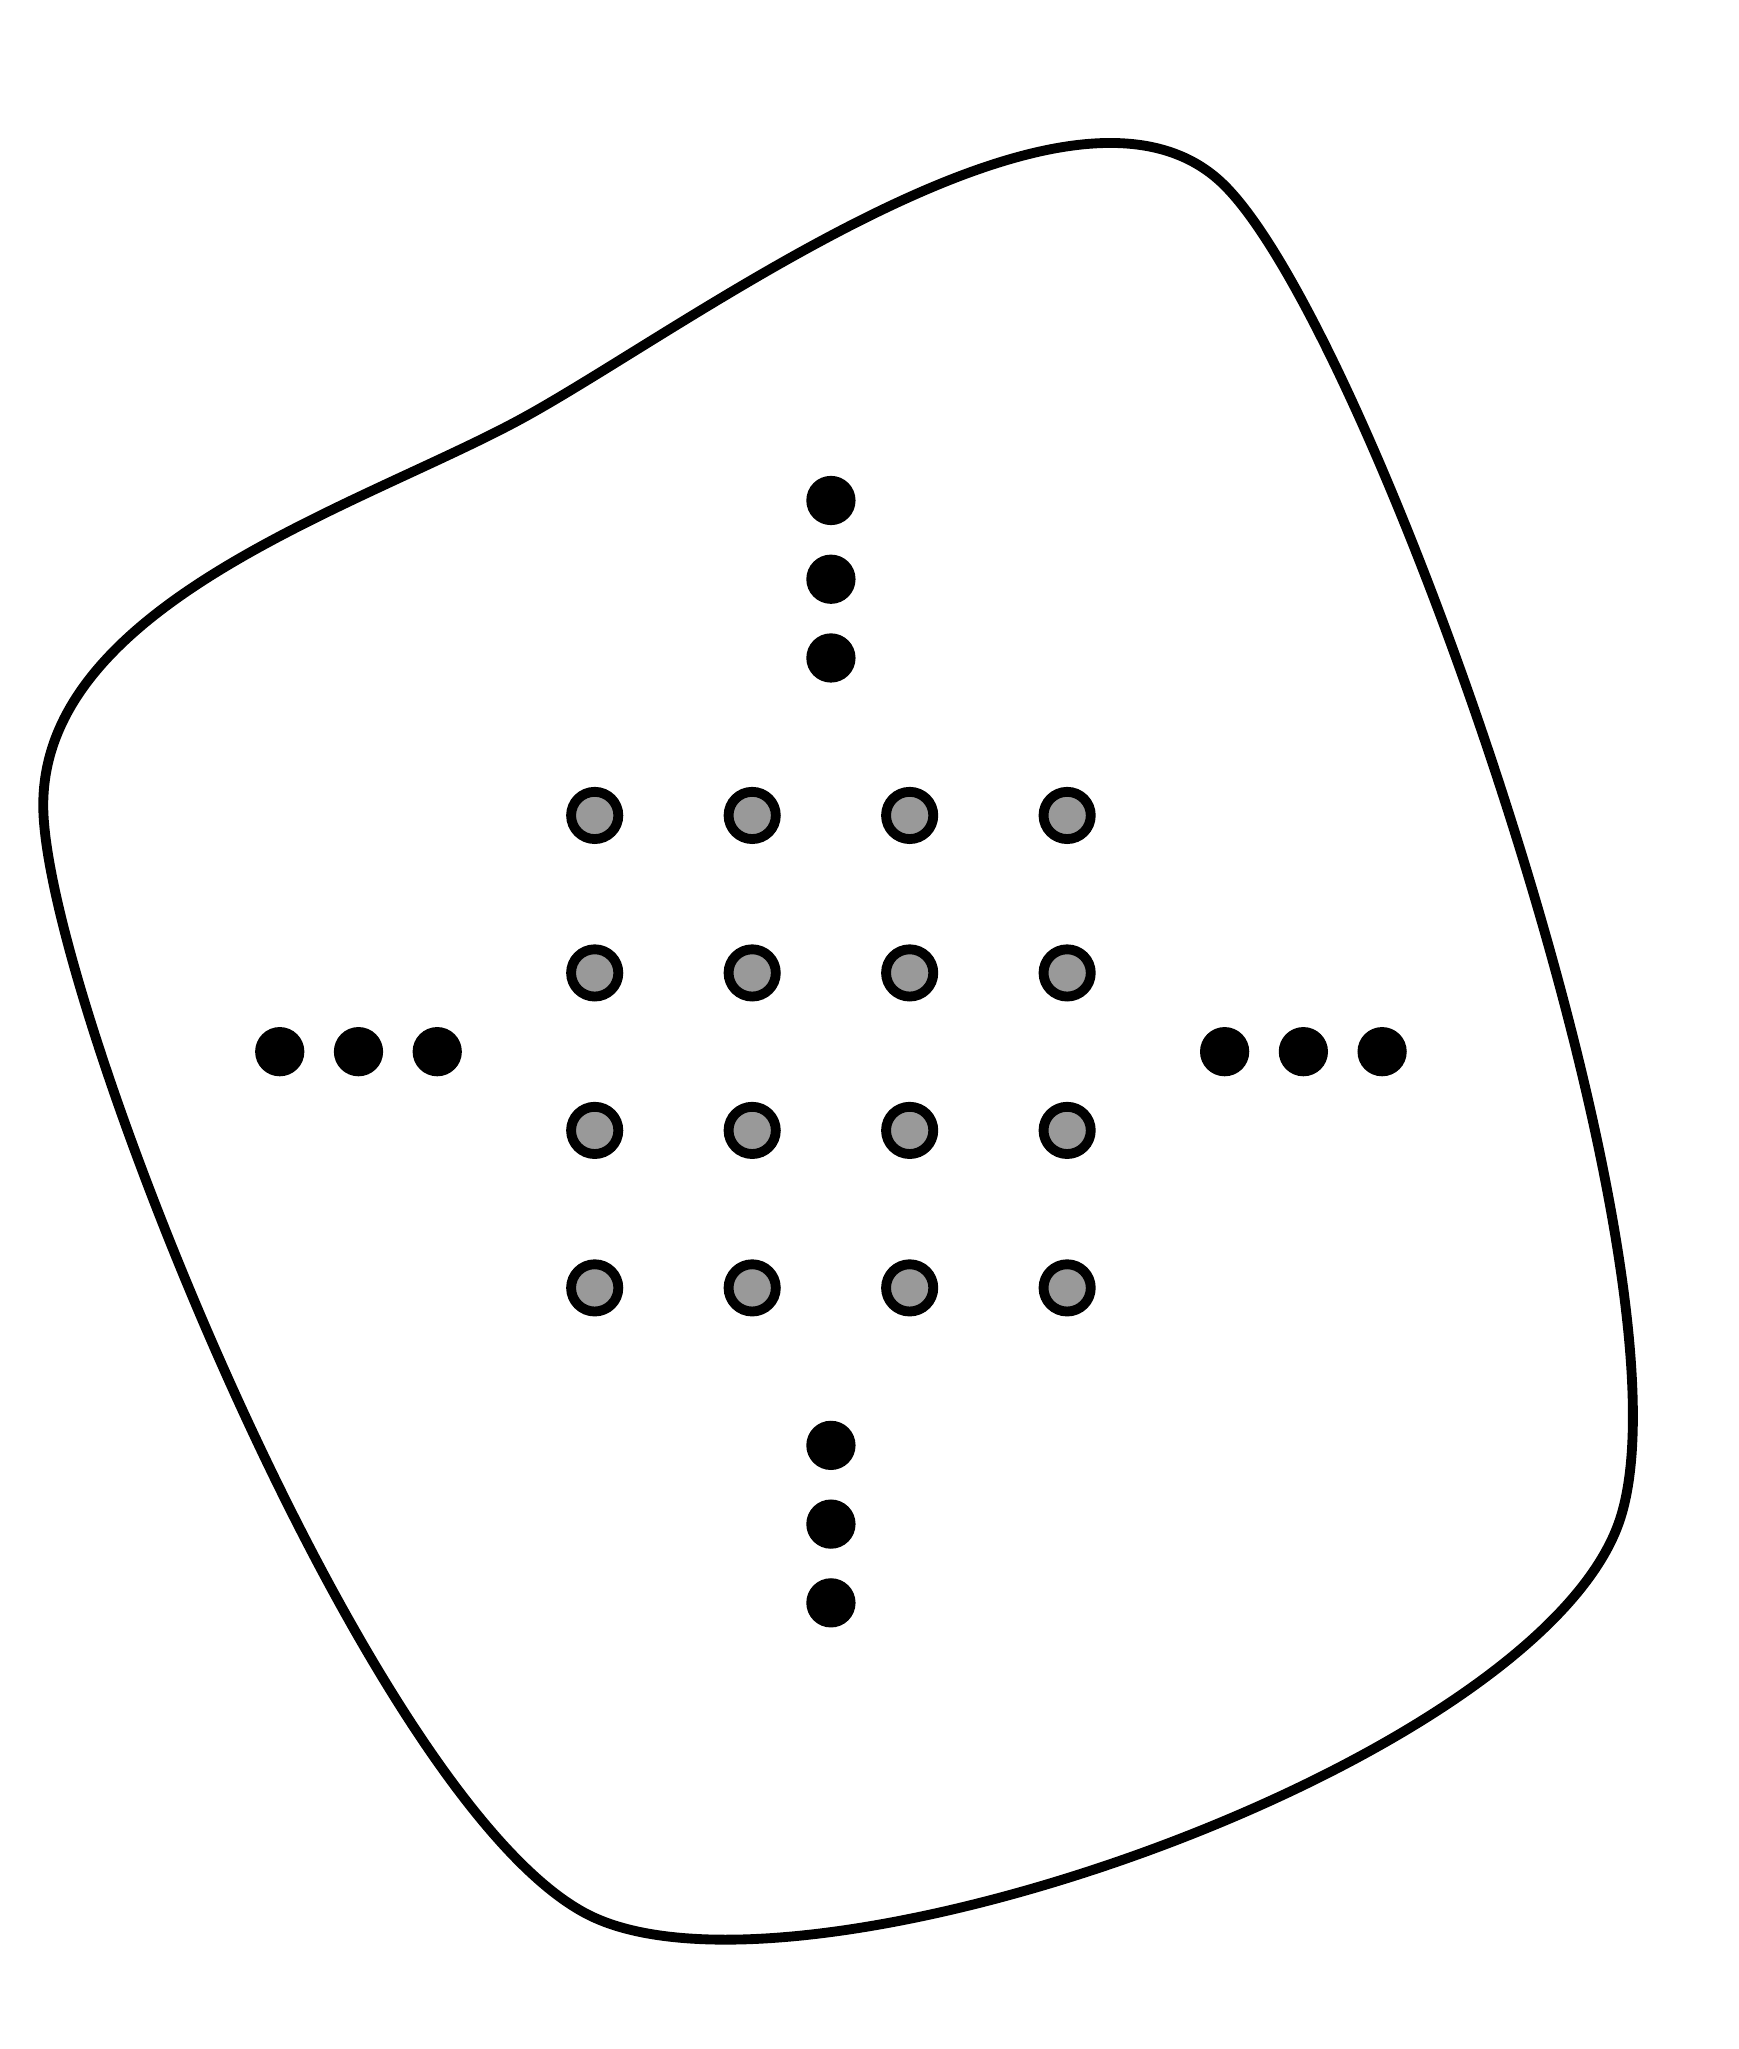
\begin{tikzpicture}[>=latex,node distance=0pt, line width=1.25mm]

    %\draw [gray!50]  (6,15)--(13,1)--(26,6)--(21,23)--(12,20) -- cycle;
    \draw [black] plot [smooth cycle] coordinates {(6,15) (13,1) (26,6) (21,23) (12,20)};

    \begin{scope}[xshift = 4cm]

    \foreach \y [count=\n]in {8,10,12,14}{ 
       \foreach \x [count=\n]in {8,10,12,14}{ 
         \begin{scope}[yshift = \y cm,xshift = \x cm,start chain=going right]
           %\draw (0,0) -- (2,0) -- (2,2) -- (0,2) -- cycle;
           \filldraw[fill=black!40!white,draw=black] (1,1) circle (0.3cm);
         \end{scope}
       }
    }

    \filldraw[fill=black,draw=black] (5,12) circle (0.25cm);
    \filldraw[fill=black,draw=black] (6,12) circle (0.25cm);
    \filldraw[fill=black,draw=black] (7,12) circle (0.25cm);

    \filldraw[fill=black,draw=black] (17,12) circle (0.25cm);
    \filldraw[fill=black,draw=black] (18,12) circle (0.25cm);
    \filldraw[fill=black,draw=black] (19,12) circle (0.25cm);

    \filldraw[fill=black,draw=black] (12,5) circle (0.25cm);
    \filldraw[fill=black,draw=black] (12,6) circle (0.25cm);
    \filldraw[fill=black,draw=black] (12,7) circle (0.25cm);

    \filldraw[fill=black,draw=black] (12,17) circle (0.25cm);
    \filldraw[fill=black,draw=black] (12,18) circle (0.25cm);
    \filldraw[fill=black,draw=black] (12,19) circle (0.25cm);

    \end{scope}

\end{tikzpicture}

\end{document}
}
\end{figure}
\end{frame}

%------------------------------------------------

\begin{frame}
\frametitle{FEM directly strategy}
\begin{figure}[!ht]
\resizebox{1.0\linewidth}{!}{\documentclass{standalone}

\begin{document}

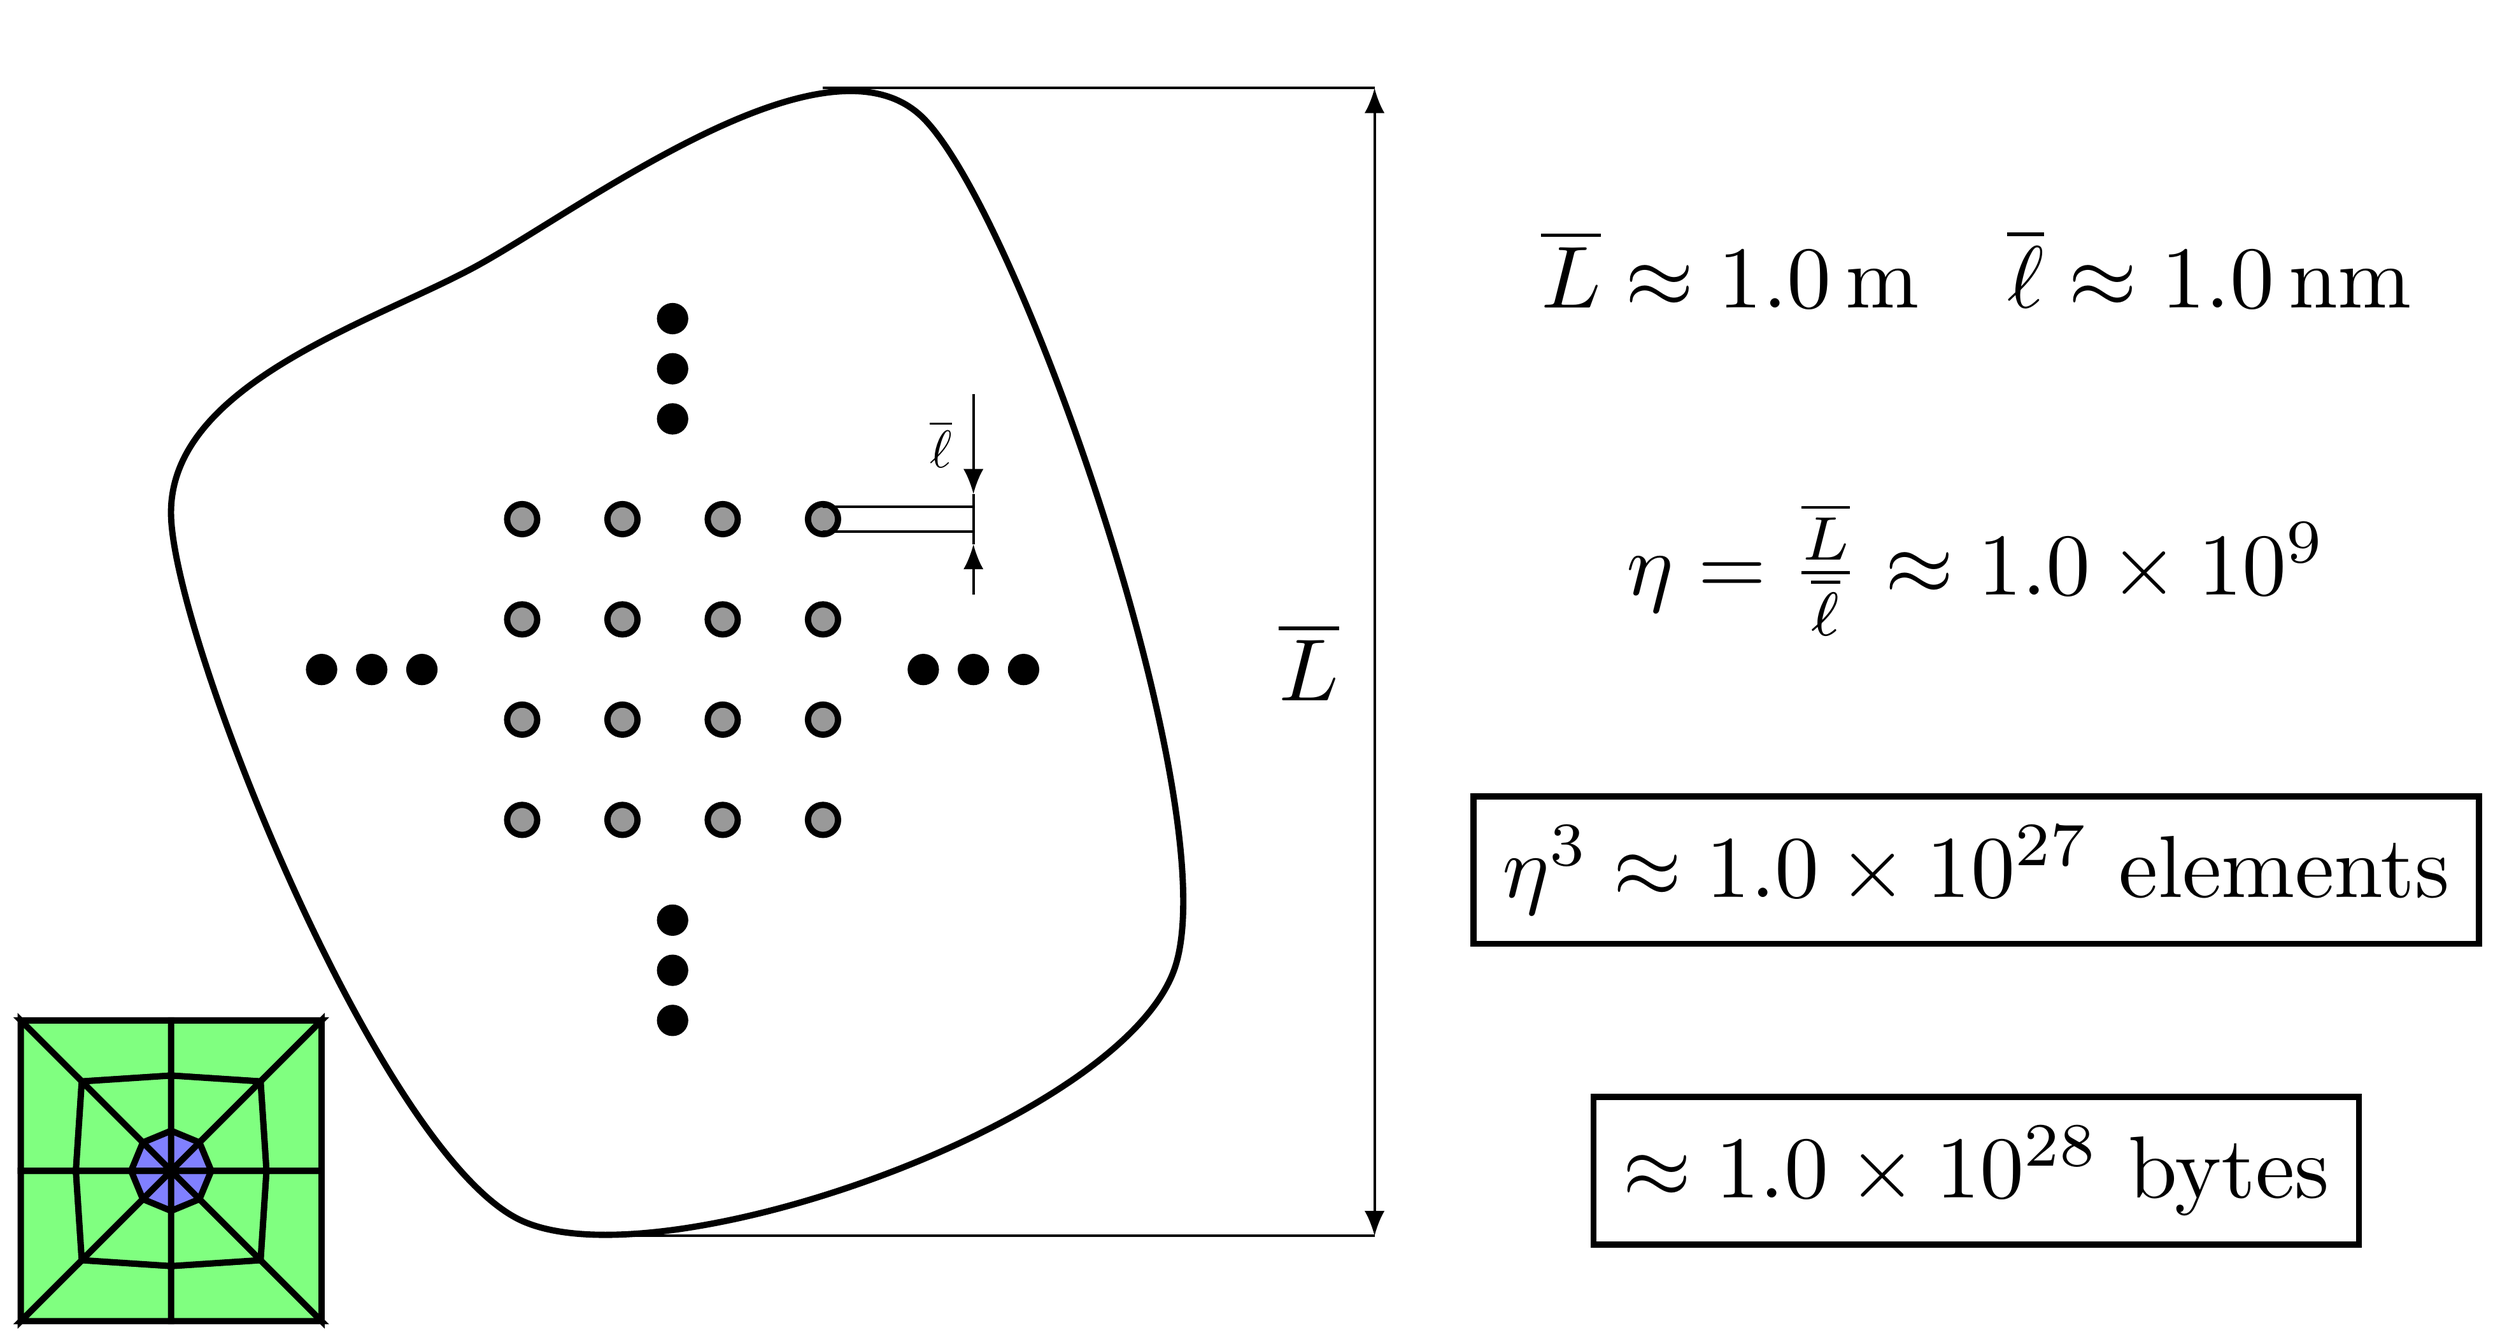
\begin{tikzpicture}[>=latex,node distance=0pt, line width=1.25mm]

    \begin{scope}[xshift=-2cm, yshift=-2cm]
    %\draw [gray!50]  (6,15)--(13,1)--(26,6)--(21,23)--(12,20) -- cycle;
    \draw [black] plot [smooth cycle] coordinates {(6,15) (13,1) (26,6) (21,23) (12,20)};

    \begin{scope}[xshift = 4 cm]

    \foreach \y [count=\n]in {8,10,12,14}{ 
       \foreach \x [count=\n]in {8,10,12,14}{ 
         \begin{scope}[yshift = \y cm,xshift = \x cm,start chain=going right]
           %\draw (0,0) -- (2,0) -- (2,2) -- (0,2) -- cycle;
           \filldraw[fill=black!40!white,draw=black] (1,1) circle (0.3cm);
         \end{scope}
       }
    }

  \draw[line width=0.5mm] (15,15.25) -- ++(3,0);
  \draw[line width=0.5mm] (15,14.75) -- ++(3,0);
  \draw[line width=0.5mm] (18,14.5) -- ++(0,1);
  \draw[{Latex[length=5mm,width=4mm]}-,line width=0.5mm] (18,14.5) -- ++(0,-1);
  \draw[{Latex[length=5mm,width=4mm]}-,line width=0.5mm] (18,15.5) --
  node[left,rotate=0,scale=3] {$\overline{\ell}$}  ++(0,2);

  %\draw[{Latex[length=5mm,width=4mm]}-{Latex[length=5mm,width=4mm]},line width=0.5mm] 
  %(30,0.7) --  node[left,rotate=0,scale=1] {$\overline{L}$} ++(0,22.9);

  \filldraw[fill=black,draw=black] (5,12) circle (0.25cm);
  \filldraw[fill=black,draw=black] (6,12) circle (0.25cm);
  \filldraw[fill=black,draw=black] (7,12) circle (0.25cm);

  \filldraw[fill=black,draw=black] (17,12) circle (0.25cm);
  \filldraw[fill=black,draw=black] (18,12) circle (0.25cm);
  \filldraw[fill=black,draw=black] (19,12) circle (0.25cm);

  \filldraw[fill=black,draw=black] (12,5) circle (0.25cm);
  \filldraw[fill=black,draw=black] (12,6) circle (0.25cm);
  \filldraw[fill=black,draw=black] (12,7) circle (0.25cm);

  \filldraw[fill=black,draw=black] (12,17) circle (0.25cm);
  \filldraw[fill=black,draw=black] (12,18) circle (0.25cm);
  \filldraw[fill=black,draw=black] (12,19) circle (0.25cm);

  \end{scope}

  \draw[line width=0.5mm] (19,23.6) -- ++(11,0);
  \draw[line width=0.5mm] (15,0.7) -- ++(15,0);
  \draw[{Latex[length=5mm,width=4mm]}-{Latex[length=5mm,width=4mm]},line width=0.5mm] 
  (30,0.7) --  node[left,rotate=0,scale=5] {$\overline{L}$} ++(0,22.9);
  \end{scope}

  \node[draw=none,fill=none,scale=5] at (40,18) {$\overline{L}\approx\SI{1.0}{\meter} \quad
  \overline{\ell}\approx\SI{1.0}{\nano\meter}$};
  \node[draw=none,fill=none,scale=5] at (40,12) {$\eta = \frac{\overline{L}}{\overline{\ell}} \approx \SI{1.0e9}{}$};
  \node[draw,fill=none,scale=5] at (40,6) {$\eta^3 \approx \SI{1.0e27}{}$ elements};
  \node[draw,fill=none,scale=5] at (40,0) {$\approx \SI{1.0e28}{}$ bytes};

  \begin{scope}[yshift = -3cm,xshift = 1cm,scale=2]
  \coordinate [draw=black,shift={(0,0)}] (0) at (0,0);
  \coordinate [draw=black,shift={(0,0)}] (1) at (1.5,0);
  \coordinate [draw=black,shift={(0,0)}] (2) at (1.5,1.5);
  \coordinate [draw=black,shift={(0,0)}] (3) at (1.5,1.1);
  \coordinate [draw=black,shift={(0,0)}] (4) at (1.2171572876,1.2171572876);
  \coordinate [draw=black,shift={(0,0)}] (5) at (1.1,1.5);
  \coordinate [draw=black,shift={(0,0)}] (6) at (0,1.5);
  \coordinate [draw=black,shift={(0,0)}] (7) at (0,3);
  \coordinate [draw=black,shift={(0,0)}] (8) at (1.2171572876,1.7828427124);
  \coordinate [draw=black,shift={(0,0)}] (9) at (1.5,1.9);
  \coordinate [draw=black,shift={(0,0)}] (10) at (1.5,3);
  \coordinate [draw=black,shift={(0,0)}] (11) at (3,0);
  \coordinate [draw=black,shift={(0,0)}] (12) at (1.7828427124,1.2171572876);
  \coordinate [draw=black,shift={(0,0)}] (13) at (1.9,1.5);
  \coordinate [draw=black,shift={(0,0)}] (14) at (3,1.5);
  \coordinate [draw=black,shift={(0,0)}] (15) at (3,3);
  \coordinate [draw=black,shift={(0,0)}] (16) at (1.7828427124,1.7828427124);
  \coordinate [draw=black,shift={(0,0)}] (17) at (1.5,0.5500000000014312);
  \coordinate [draw=black,shift={(0,0)}] (18) at (0.6085786437983935,0.6085786437983935);
  \coordinate [draw=black,shift={(0,0)}] (19) at (0.5500000000014312,1.5);
  \coordinate [draw=black,shift={(0,0)}] (20) at (0.6085786437983723,2.391421356201628);
  \coordinate [draw=black,shift={(0,0)}] (21) at (1.5,2.449999999998004);
  \coordinate [draw=black,shift={(0,0)}] (22) at (2.391421356201628,0.6085786437983723);
  \coordinate [draw=black,shift={(0,0)}] (23) at (2.449999999998004,1.5);
  \coordinate [draw=black,shift={(0,0)}] (24) at (2.391421356201648,2.391421356201648);
  \draw [fill=blue!50] (2) --  (4) --  (3) -- cycle;
  \draw [fill=blue!50] (2) --  (4) --  (5) -- cycle;
  \draw [fill=blue!50] (2) --  (8) --  (9) -- cycle;
  \draw [fill=blue!50] (2) --  (8) --  (5) -- cycle;
  \draw [fill=blue!50] (2) --  (12) --  (3) -- cycle;
  \draw [fill=blue!50] (2) --  (12) --  (13) -- cycle;
  \draw [fill=blue!50] (2) --  (16) --  (9) -- cycle;
  \draw [fill=blue!50] (2) --  (16) --  (13) -- cycle;
  \draw [fill=green!50] (0) --  (18) --  (17) --  (1) -- cycle;
  \draw [fill=green!50] (18) --  (4) --  (3) --  (17) -- cycle;
  \draw [fill=green!50] (0) --  (18) --  (19) --  (6) -- cycle;
  \draw [fill=green!50] (18) --  (4) --  (5) --  (19) -- cycle;
  \draw [fill=green!50] (7) --  (20) --  (21) --  (10) -- cycle;
  \draw [fill=green!50] (20) --  (8) --  (9) --  (21) -- cycle;
  \draw [fill=green!50] (7) --  (20) --  (19) --  (6) -- cycle;
  \draw [fill=green!50] (20) --  (8) --  (5) --  (19) -- cycle;
  \draw [fill=green!50] (11) --  (22) --  (17) --  (1) -- cycle;
  \draw [fill=green!50] (22) --  (12) --  (3) --  (17) -- cycle;
  \draw [fill=green!50] (11) --  (22) --  (23) --  (14) -- cycle;
  \draw [fill=green!50] (22) --  (12) --  (13) --  (23) -- cycle;
  \draw [fill=green!50] (15) --  (24) --  (21) --  (10) -- cycle;
  \draw [fill=green!50] (24) --  (16) --  (9) --  (21) -- cycle;
  \draw [fill=green!50] (15) --  (24) --  (23) --  (14) -- cycle;
  \draw [fill=green!50] (24) --  (16) --  (13) --  (23) -- cycle;
  \node [fill=black, draw=none, circle, inner sep=0pt, minimum size=0.1cm,scale=0.3] at (0) {h};
  \node [fill=black, draw=none, circle, inner sep=0pt, minimum size=0.1cm,scale=0.3] at (1) {h};
  \node [fill=black, draw=none, circle, inner sep=0pt, minimum size=0.1cm,scale=0.3] at (2) {h};
  \node [fill=black, draw=none, circle, inner sep=0pt, minimum size=0.1cm,scale=0.3] at (3) {h};
  \node [fill=black, draw=none, circle, inner sep=0pt, minimum size=0.1cm,scale=0.3] at (4) {h};
  \node [fill=black, draw=none, circle, inner sep=0pt, minimum size=0.1cm,scale=0.3] at (5) {h};
  \node [fill=black, draw=none, circle, inner sep=0pt, minimum size=0.1cm,scale=0.3] at (6) {h};
  \node [fill=black, draw=none, circle, inner sep=0pt, minimum size=0.1cm,scale=0.3] at (7) {h};
  \node [fill=black, draw=none, circle, inner sep=0pt, minimum size=0.1cm,scale=0.3] at (8) {h};
  \node [fill=black, draw=none, circle, inner sep=0pt, minimum size=0.1cm,scale=0.3] at (9) {h};
  \node [fill=black, draw=none, circle, inner sep=0pt, minimum size=0.1cm,scale=0.3] at (10) {h};
  \node [fill=black, draw=none, circle, inner sep=0pt, minimum size=0.1cm,scale=0.3] at (11) {h};
  \node [fill=black, draw=none, circle, inner sep=0pt, minimum size=0.1cm,scale=0.3] at (12) {h};
  \node [fill=black, draw=none, circle, inner sep=0pt, minimum size=0.1cm,scale=0.3] at (13) {h};
  \node [fill=black, draw=none, circle, inner sep=0pt, minimum size=0.1cm,scale=0.3] at (14) {h};
  \node [fill=black, draw=none, circle, inner sep=0pt, minimum size=0.1cm,scale=0.3] at (15) {h};
  \node [fill=black, draw=none, circle, inner sep=0pt, minimum size=0.1cm,scale=0.3] at (16) {h};
  \node [fill=black, draw=none, circle, inner sep=0pt, minimum size=0.1cm,scale=0.3] at (17) {h};
  \node [fill=black, draw=none, circle, inner sep=0pt, minimum size=0.1cm,scale=0.3] at (18) {h};
  \node [fill=black, draw=none, circle, inner sep=0pt, minimum size=0.1cm,scale=0.3] at (19) {h};
  \node [fill=black, draw=none, circle, inner sep=0pt, minimum size=0.1cm,scale=0.3] at (20) {h};
  \node [fill=black, draw=none, circle, inner sep=0pt, minimum size=0.1cm,scale=0.3] at (21) {h};
  \node [fill=black, draw=none, circle, inner sep=0pt, minimum size=0.1cm,scale=0.3] at (22) {h};
  \node [fill=black, draw=none, circle, inner sep=0pt, minimum size=0.1cm,scale=0.3] at (23) {h};
  \node [fill=black, draw=none, circle, inner sep=0pt, minimum size=0.1cm,scale=0.3] at (24) {h};
  \end{scope}

\end{tikzpicture}

\end{document}

}
\end{figure}
\end{frame}

%------------------------------------------------

\begin{frame}
\frametitle{Multi-scale methods}
\begin{figure}[!ht]
\resizebox{1.0\linewidth}{!}{\documentclass{standalone}

\begin{document}

\tikzset{cross/.style={cross out, draw=black, fill=none, minimum size=2*(#1-\pgflinewidth), inner sep=0pt, outer
sep=0pt}, cross/.default={2pt}}

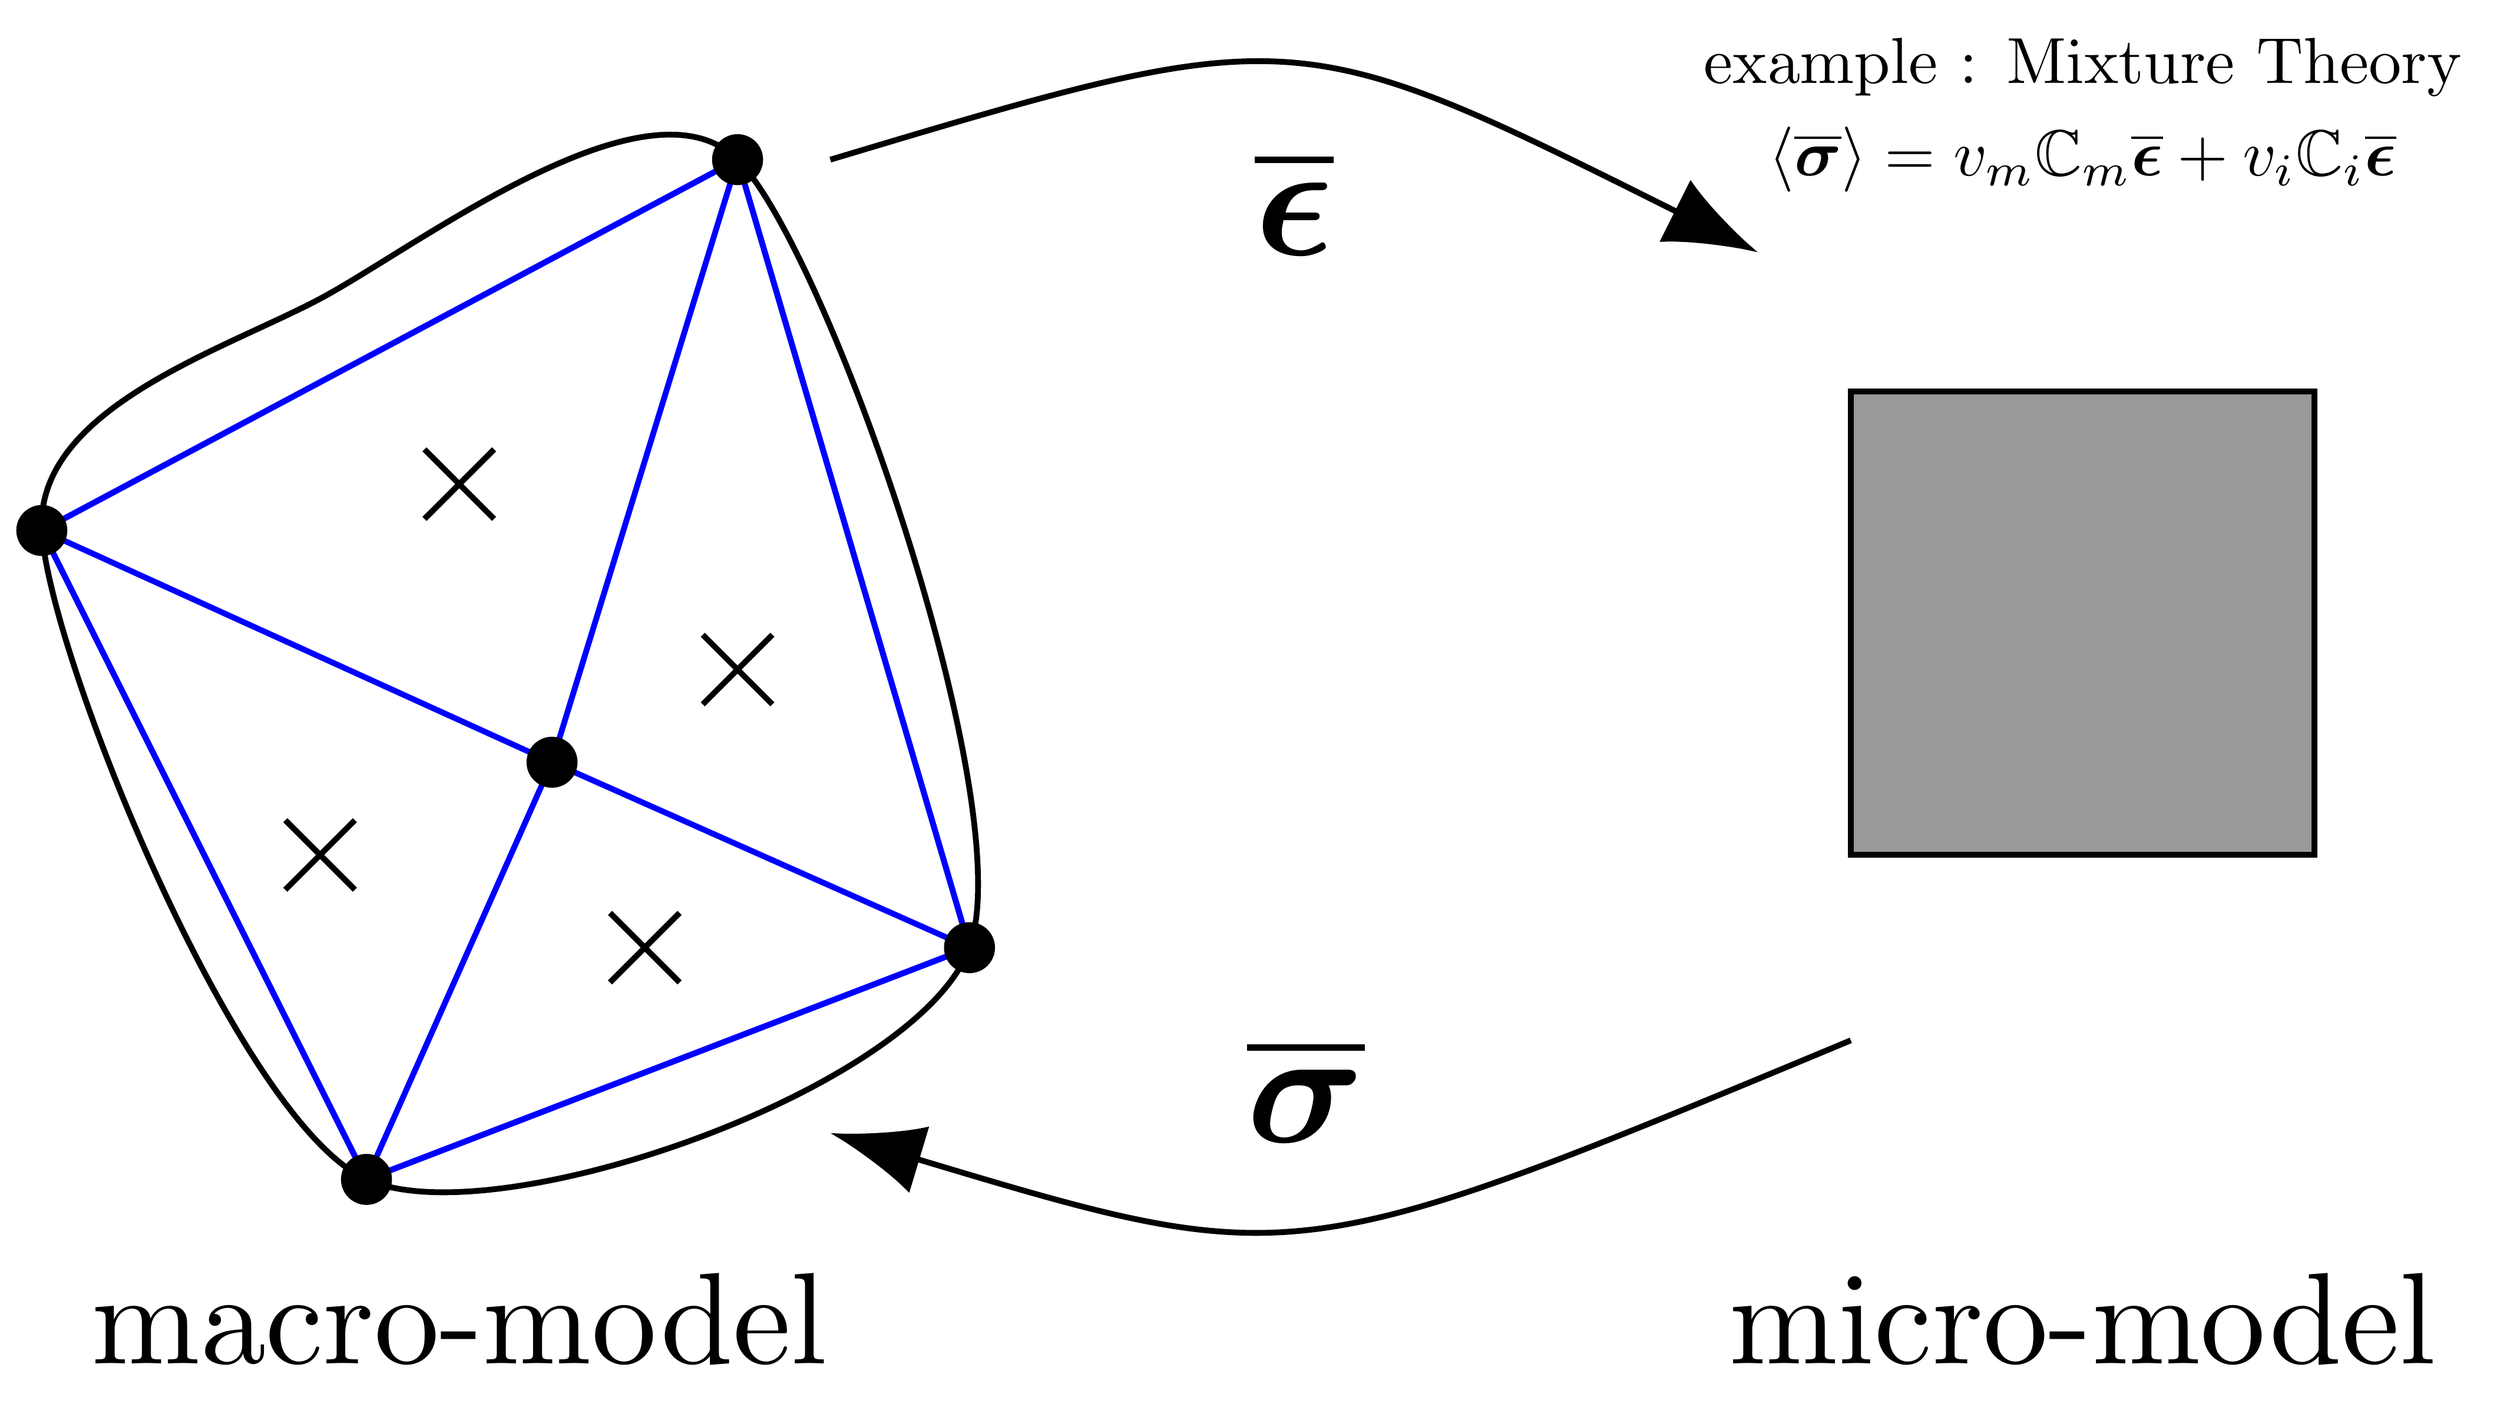
\begin{tikzpicture}[>=latex,node distance=0pt, line width=1.25mm]

% the h.m.s.

    \coordinate [draw=black,shift={(0,0)}] (0) at (6,15);
    \coordinate [draw=black,shift={(0,0)}] (1) at (13,1);
    \coordinate [draw=black,shift={(0,0)}] (2) at (26,6);
    \coordinate [draw=black,shift={(0,0)}] (3) at (21,23);
    \coordinate [draw=black,shift={(0,0)}] (4) at (17,10);
    \draw [blue]  (0) -- (1) -- (2) -- (3) -- cycle;
    \draw [blue]  (0) -- (4);
    \draw [blue]  (1) -- (4);
    \draw [blue]  (2) -- (4);
    \draw [blue]  (3) -- (4);
    \draw [blue]  (6,15) -- (13,1) -- (26,6) -- (21,23) -- cycle;
    \draw [black] plot [smooth cycle] coordinates {(6,15) (13,1) (26,6) (21,23)
    (12,20)};
    \node [fill=black, draw=none, circle, inner sep=0pt, minimum size=1.1cm,scale=1.0] at (0) {};
    \node [fill=black, draw=none, circle, inner sep=0pt, minimum size=1.1cm,scale=1.0] at (1) {};
    \node [fill=black, draw=none, circle, inner sep=0pt, minimum size=1.1cm,scale=1.0] at (2) {};
    \node [fill=black, draw=none, circle, inner sep=0pt, minimum size=1.1cm,scale=1.0] at (3) {};
    \node [fill=black, draw=none, circle, inner sep=0pt, minimum size=1.1cm,scale=1.0] at (4) {};
    \node[cross,minimum size=1.0cm,scale=1.5] (gp_0) at (12,8) {};
    \node[cross,minimum size=1.0cm,scale=1.5] (gp_0) at (15,16) {};
    \node[cross,minimum size=1.0cm,scale=1.5] (gp_0) at (19,6) {};
    \node[cross,minimum size=1.0cm,scale=1.5] (gp_0) at (21,12) {};

% the r.v.e.

    \begin{scope}[yshift = 8 cm,xshift = 45 cm,start chain=going right,scale=5]
          \filldraw[fill=black!40!white,draw=black] (0,0) -- (2,0) -- (2,2) -- (0,2) -- cycle;
    \end{scope}

    \draw[-{Latex[length=20mm,width=15mm]}] (23,23) ..  controls ++(10,+3) ..
    node[below, scale=10] {$\overline{\bm{\epsilon}}$} 
    ++(20,-2);
    \draw[{Latex[length=20mm,width=15mm]}-] (23,2) .. controls ++(10,-3) .. 
    node[above, scale=10] {$\overline{\bm{\sigma}}$}
    ++(22,+2);

    \node[scale=8] at (15,-2) {macro-model} ;
    \node[scale=8] at (50,-2) {micro-model};
    \node[scale=4] at (50,25) {example : Mixture Theory};
    \node[scale=4] at (50,23) {$\langle\overline{\bm{\sigma}}\rangle 
    = v_m \mathbb{C}_m\overline{\bm{\epsilon}} + v_i \mathbb{C}_i\overline{\bm{\epsilon}}$};


\end{tikzpicture}

\end{document}

}
\end{figure}
\end{frame}

%------------------------------------------------

\begin{frame}
\frametitle{The FE$^2$ multi-scale method}
\begin{figure}[!ht]
\resizebox{1.0\linewidth}{!}{\input{figures/multiscale_fe2.tikz}}
\end{figure}
\end{frame}

%------------------------------------------------

\begin{frame}
\frametitle{The micro-problem in the FE$^2$ method}
\begin{figure}[!ht]
\resizebox{0.8\linewidth}{!}{\input{figures/micro_eqs_a.tikz}}
\end{figure}
\end{frame}

%------------------------------------------------

\begin{frame}
\frametitle{A simple analogy}
\begin{figure}[!ht]
\resizebox{0.8\linewidth}{!}{\documentclass{standalone}

\begin{document}

\tikzset{cross/.style={cross out, draw=black, fill=none, minimum size=2*(#1-\pgflinewidth), inner sep=0pt, outer
sep=0pt}, cross/.default={2pt}}

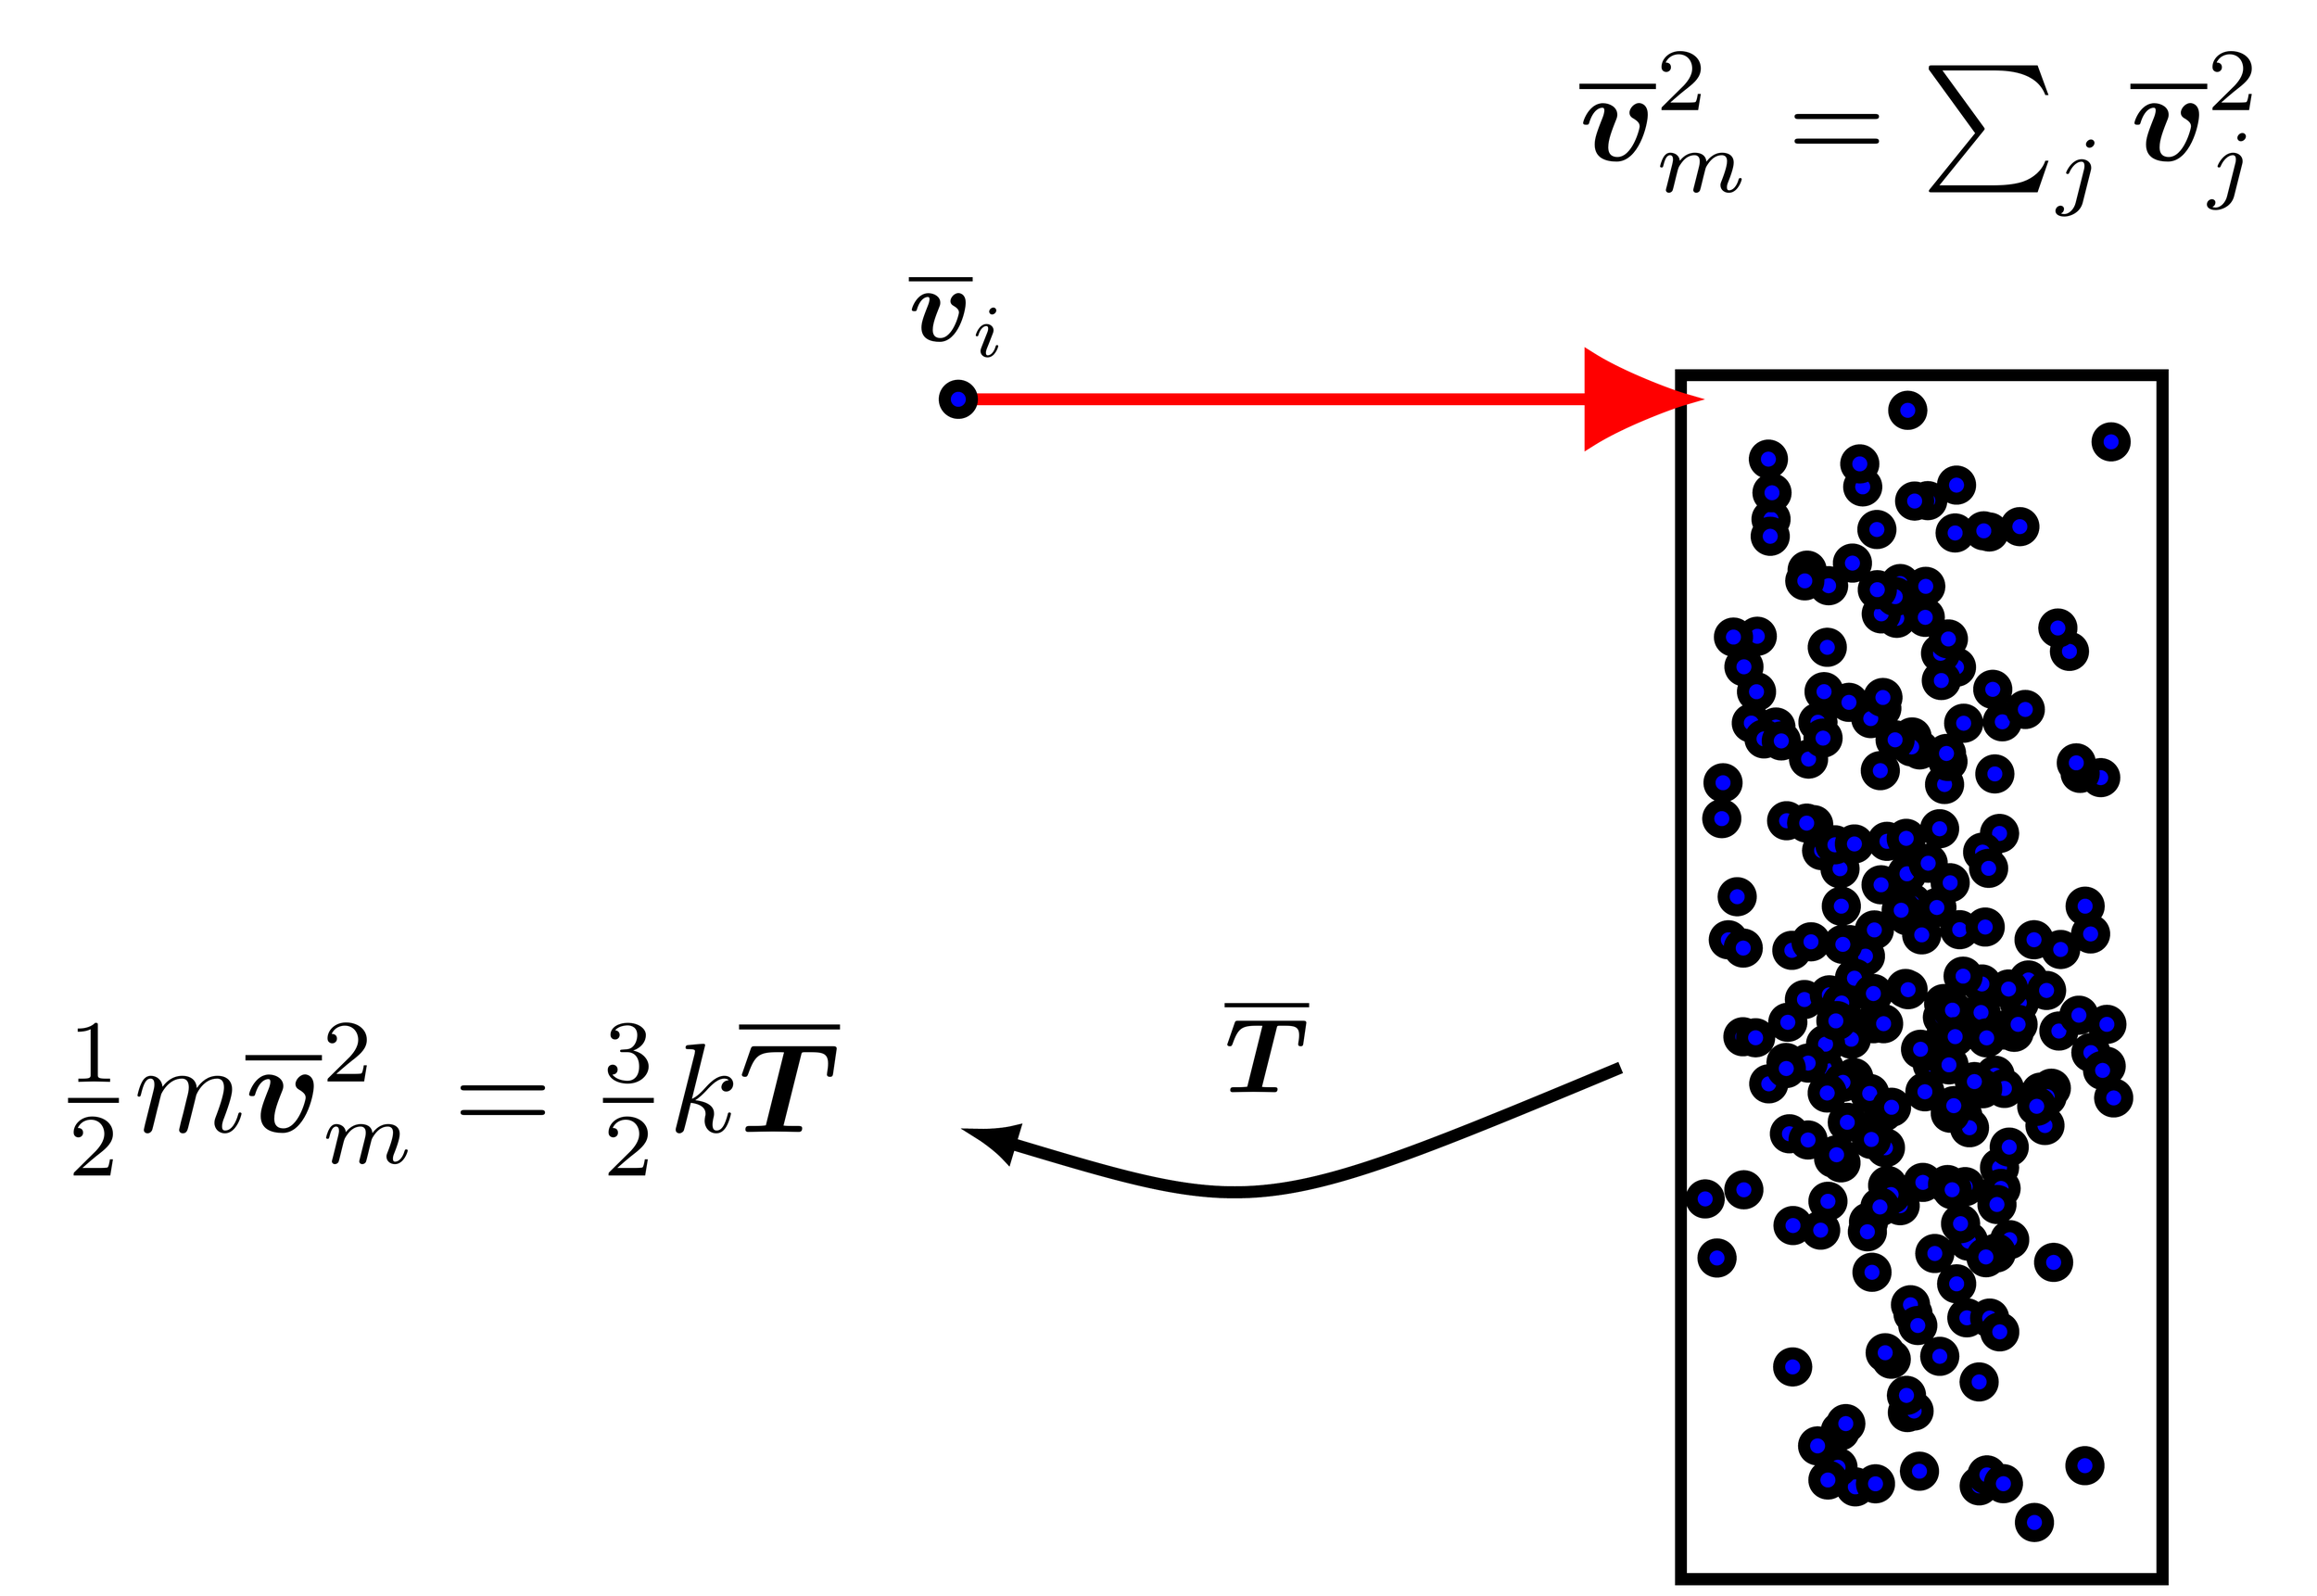
\begin{tikzpicture}[>=latex,node distance=0pt, line width=4mm]

    \begin{scope}[yshift=7 cm, xshift=40cm, start chain=going right, scale=4.0]
      \draw [fill=none] (-2,-5) --  (2,-5) --  (2,5) -- (-2,5) -- cycle;

     \foreach \d in {1,2,3}{
      \foreach \y in {2,4,5,7,8,8.2,8.5,9,9.5,9}{
       \foreach \x in {2,4,5,7,8,8.5,9,9}{
        \node [fill=blue, draw=black, circle, inner sep=0pt, minimum size=0.3cm,scale=3] at (rand*\x*0.2,rand*\y*0.5) {};
       }
      }
     } 
     \node [fill=none, draw=none, inner sep=0pt, minimum size=0.3cm,scale=10] at (-8.0,+5.5) {$\overline{\bm{v}}_i$};
     \draw[-{Latex[length=40mm,width=35mm]},draw=Red] (-8.0,+4.8) -- (-1.8,+4.8) ;
     \node [fill=blue, draw=black, circle, inner sep=0pt, minimum size=0.3cm,scale=3] at (-8.0,+4.8) {};
    \end{scope}

    \draw[{Latex[length=20mm,width=15mm]}-] (8,2) .. controls ++(10,-3) .. 
    node[above, scale=10] {$\overline{\bm{T}}$}
    ++(22,+2);

    \node[scale=12] at (-9,3) {$\frac{1}{2}m\overline{\bm{v}}_{m}^2 = \frac{3}{2}k\overline{\bm{T}}$};
    \node[scale=12] at (40,35) {$\overline{\bm{v}}_{m}^2 = \sum_j \overline{\bm{v}}_j^2$};

\end{tikzpicture}

\end{document}

}
\end{figure}
\end{frame}

%------------------------------------------------

\begin{frame}
\frametitle{The micro-problem in the FE$^2$ method}
\begin{figure}[!ht]
\resizebox{0.8\linewidth}{!}{\documentclass{standalone}

\begin{document}

\tikzset{cross/.style={cross out, draw=black, fill=none, minimum size=2*(#1-\pgflinewidth), inner sep=0pt, outer
sep=0pt}, cross/.default={2pt}}

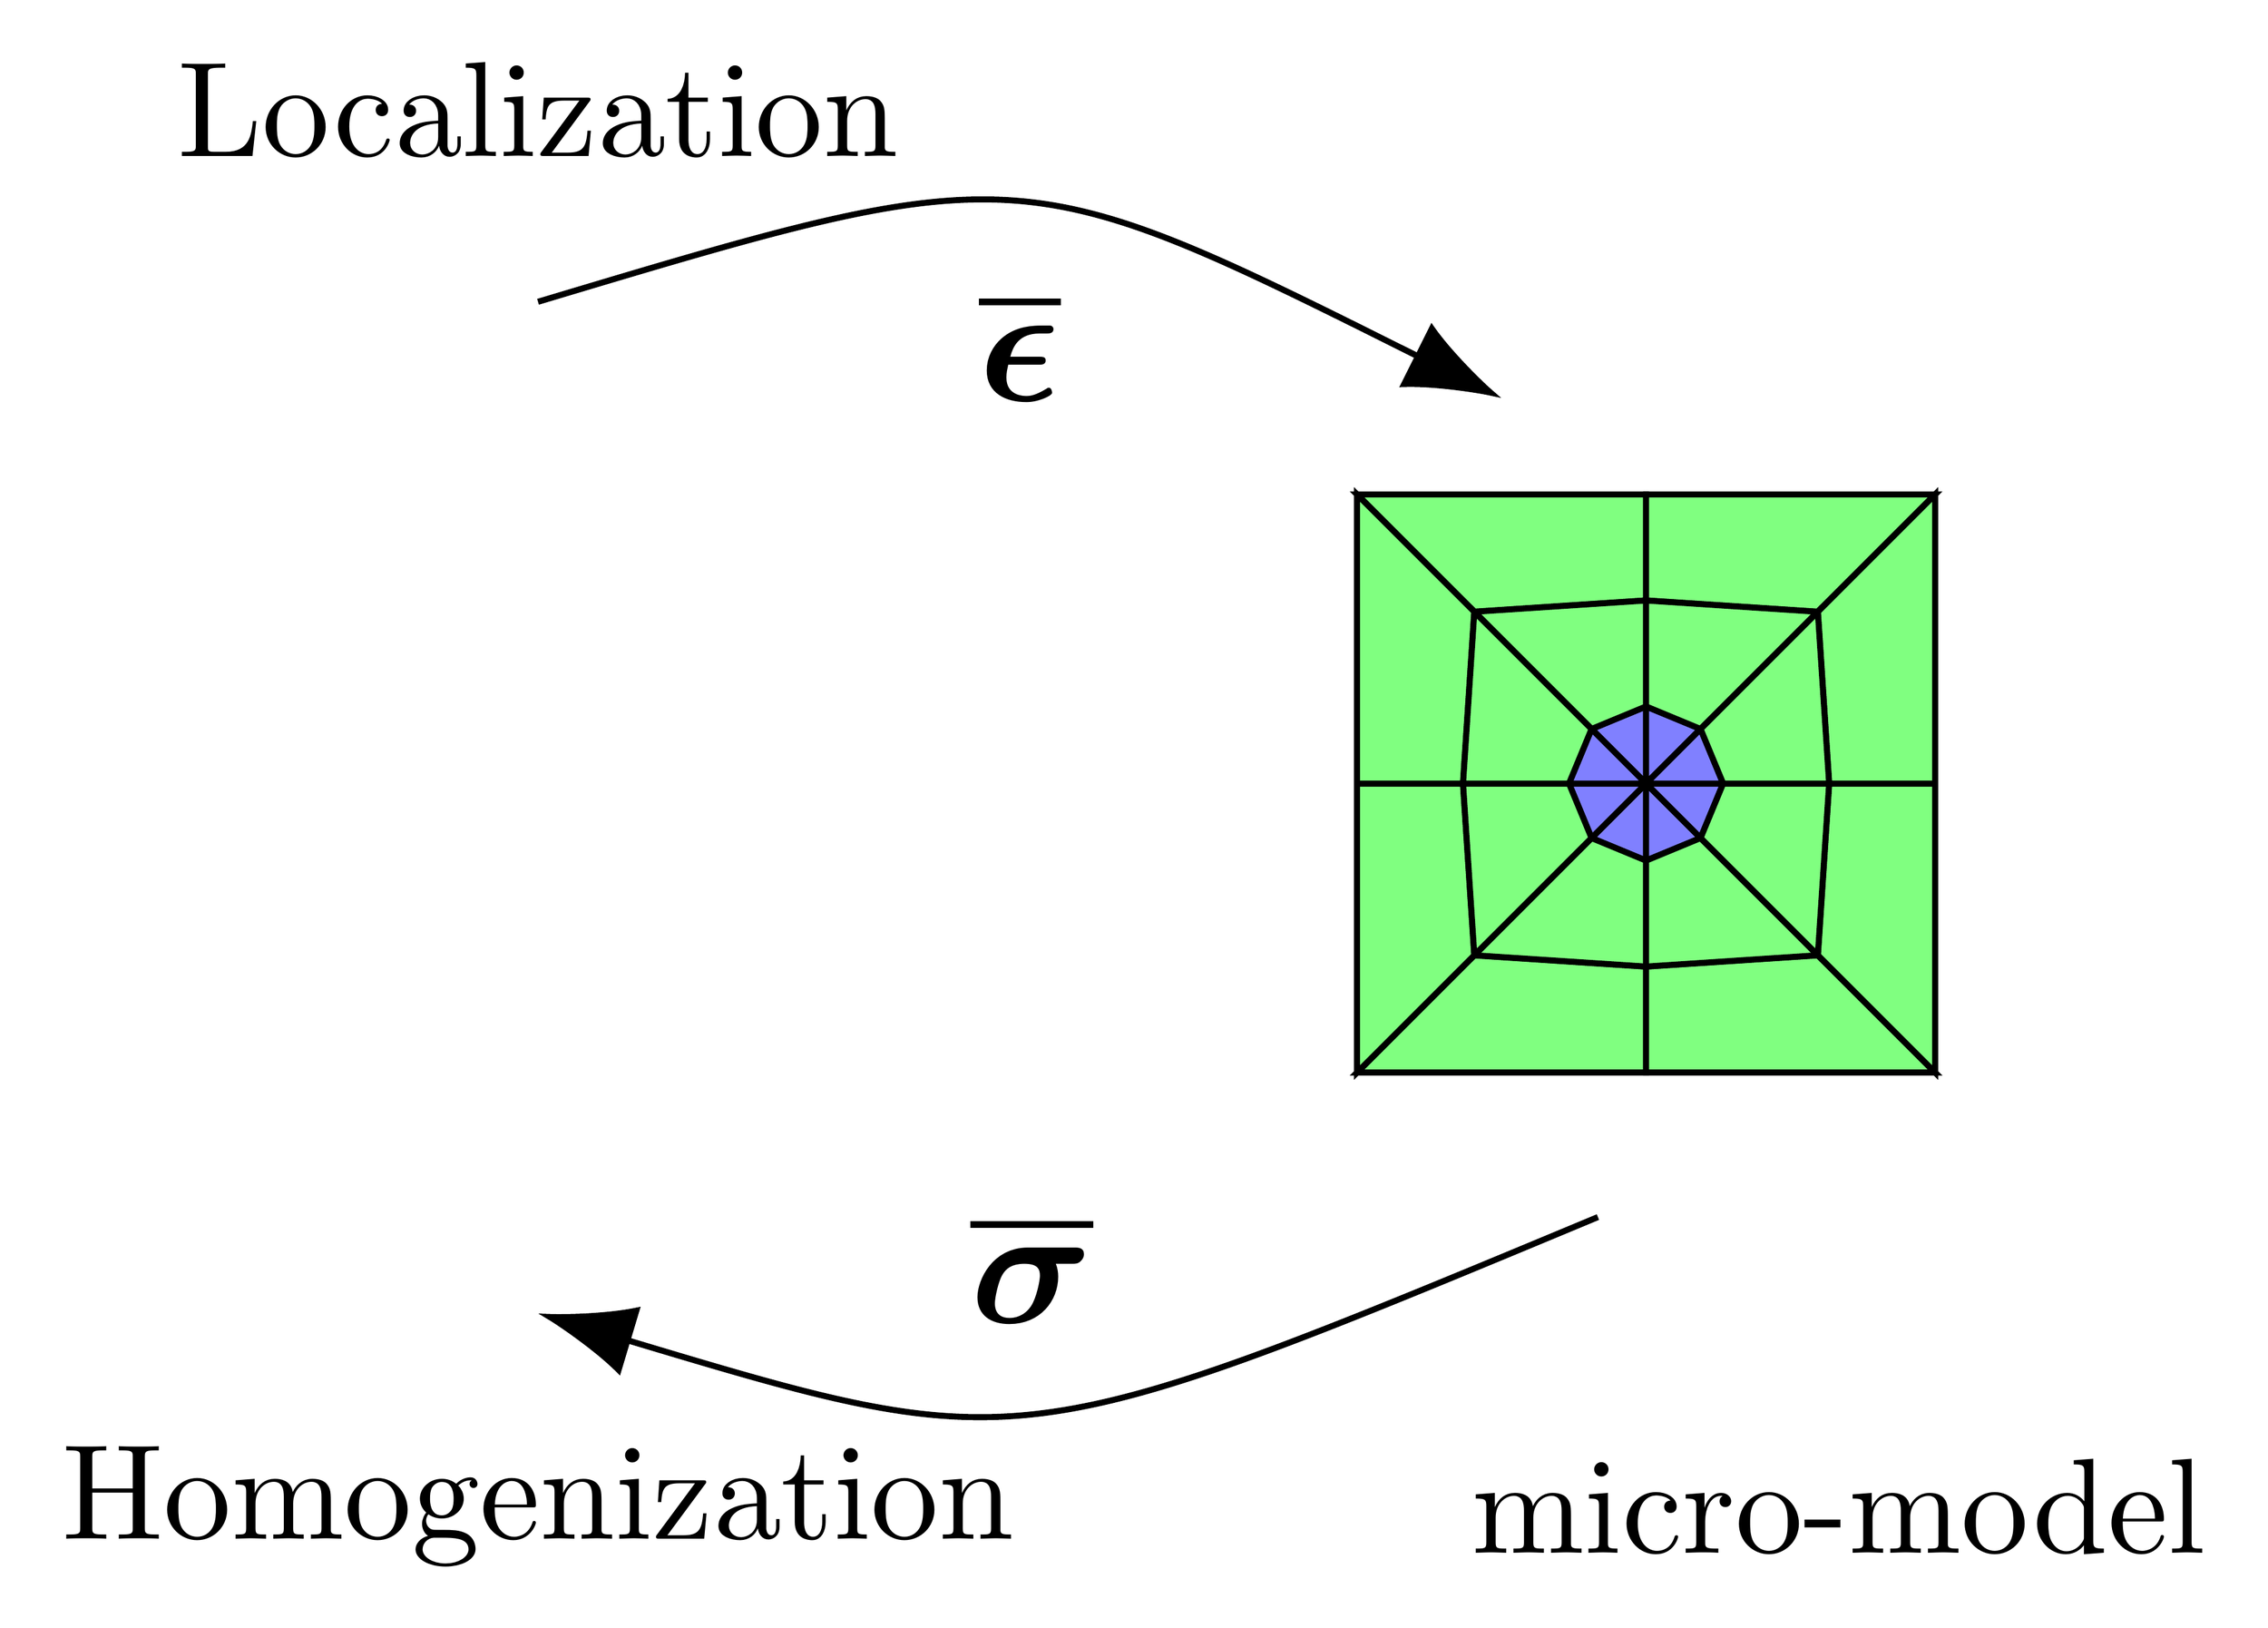
\begin{tikzpicture}[>=latex,node distance=0pt, line width=1.25mm]

    \begin{scope}[yshift=7 cm, xshift=40cm, start chain=going right, scale=4.0]
      \coordinate [draw=black,shift={(0,0)}] (0) at (0,0);
      \coordinate [draw=black,shift={(0,0)}] (1) at (1.5,0);
      \coordinate [draw=black,shift={(0,0)}] (2) at (1.5,1.5);
      \coordinate [draw=black,shift={(0,0)}] (3) at (1.5,1.1);
      \coordinate [draw=black,shift={(0,0)}] (4) at (1.2171572876,1.2171572876);
      \coordinate [draw=black,shift={(0,0)}] (5) at (1.1,1.5);
      \coordinate [draw=black,shift={(0,0)}] (6) at (0,1.5);
      \coordinate [draw=black,shift={(0,0)}] (7) at (0,3);
      \coordinate [draw=black,shift={(0,0)}] (8) at (1.2171572876,1.7828427124);
      \coordinate [draw=black,shift={(0,0)}] (9) at (1.5,1.9);
      \coordinate [draw=black,shift={(0,0)}] (10) at (1.5,3);
      \coordinate [draw=black,shift={(0,0)}] (11) at (3,0);
      \coordinate [draw=black,shift={(0,0)}] (12) at (1.7828427124,1.2171572876);
      \coordinate [draw=black,shift={(0,0)}] (13) at (1.9,1.5);
      \coordinate [draw=black,shift={(0,0)}] (14) at (3,1.5);
      \coordinate [draw=black,shift={(0,0)}] (15) at (3,3);
      \coordinate [draw=black,shift={(0,0)}] (16) at (1.7828427124,1.7828427124);
      \coordinate [draw=black,shift={(0,0)}] (17) at (1.5,0.5500000000014312);
      \coordinate [draw=black,shift={(0,0)}] (18) at (0.6085786437983935,0.6085786437983935);
      \coordinate [draw=black,shift={(0,0)}] (19) at (0.5500000000014312,1.5);
      \coordinate [draw=black,shift={(0,0)}] (20) at (0.6085786437983723,2.391421356201628);
      \coordinate [draw=black,shift={(0,0)}] (21) at (1.5,2.449999999998004);
      \coordinate [draw=black,shift={(0,0)}] (22) at (2.391421356201628,0.6085786437983723);
      \coordinate [draw=black,shift={(0,0)}] (23) at (2.449999999998004,1.5);
      \coordinate [draw=black,shift={(0,0)}] (24) at (2.391421356201648,2.391421356201648);
      \draw [fill=blue!50] (2) --  (4) --  (3) -- cycle;
      \draw [fill=blue!50] (2) --  (4) --  (5) -- cycle;
      \draw [fill=blue!50] (2) --  (8) --  (9) -- cycle;
      \draw [fill=blue!50] (2) --  (8) --  (5) -- cycle;
      \draw [fill=blue!50] (2) --  (12) --  (3) -- cycle;
      \draw [fill=blue!50] (2) --  (12) --  (13) -- cycle;
      \draw [fill=blue!50] (2) --  (16) --  (9) -- cycle;
      \draw [fill=blue!50] (2) --  (16) --  (13) -- cycle;
      \draw [fill=green!50] (0) --  (18) --  (17) --  (1) -- cycle;
      \draw [fill=green!50] (18) --  (4) --  (3) --  (17) -- cycle;
      \draw [fill=green!50] (0) --  (18) --  (19) --  (6) -- cycle;
      \draw [fill=green!50] (18) --  (4) --  (5) --  (19) -- cycle;
      \draw [fill=green!50] (7) --  (20) --  (21) --  (10) -- cycle;
      \draw [fill=green!50] (20) --  (8) --  (9) --  (21) -- cycle;
      \draw [fill=green!50] (7) --  (20) --  (19) --  (6) -- cycle;
      \draw [fill=green!50] (20) --  (8) --  (5) --  (19) -- cycle;
      \draw [fill=green!50] (11) --  (22) --  (17) --  (1) -- cycle;
      \draw [fill=green!50] (22) --  (12) --  (3) --  (17) -- cycle;
      \draw [fill=green!50] (11) --  (22) --  (23) --  (14) -- cycle;
      \draw [fill=green!50] (22) --  (12) --  (13) --  (23) -- cycle;
      \draw [fill=green!50] (15) --  (24) --  (21) --  (10) -- cycle;
      \draw [fill=green!50] (24) --  (16) --  (9) --  (21) -- cycle;
      \draw [fill=green!50] (15) --  (24) --  (23) --  (14) -- cycle;
      \draw [fill=green!50] (24) --  (16) --  (13) --  (23) -- cycle;
      \node [fill=black, draw=none, circle, inner sep=0pt, minimum size=0.1cm,scale=0.3] at (0) {h};
      \node [fill=black, draw=none, circle, inner sep=0pt, minimum size=0.1cm,scale=0.3] at (1) {h};
      \node [fill=black, draw=none, circle, inner sep=0pt, minimum size=0.1cm,scale=0.3] at (2) {h};
      \node [fill=black, draw=none, circle, inner sep=0pt, minimum size=0.1cm,scale=0.3] at (3) {h};
      \node [fill=black, draw=none, circle, inner sep=0pt, minimum size=0.1cm,scale=0.3] at (4) {h};
      \node [fill=black, draw=none, circle, inner sep=0pt, minimum size=0.1cm,scale=0.3] at (5) {h};
      \node [fill=black, draw=none, circle, inner sep=0pt, minimum size=0.1cm,scale=0.3] at (6) {h};
      \node [fill=black, draw=none, circle, inner sep=0pt, minimum size=0.1cm,scale=0.3] at (7) {h};
      \node [fill=black, draw=none, circle, inner sep=0pt, minimum size=0.1cm,scale=0.3] at (8) {h};
      \node [fill=black, draw=none, circle, inner sep=0pt, minimum size=0.1cm,scale=0.3] at (9) {h};
      \node [fill=black, draw=none, circle, inner sep=0pt, minimum size=0.1cm,scale=0.3] at (10) {h};
      \node [fill=black, draw=none, circle, inner sep=0pt, minimum size=0.1cm,scale=0.3] at (11) {h};
      \node [fill=black, draw=none, circle, inner sep=0pt, minimum size=0.1cm,scale=0.3] at (12) {h};
      \node [fill=black, draw=none, circle, inner sep=0pt, minimum size=0.1cm,scale=0.3] at (13) {h};
      \node [fill=black, draw=none, circle, inner sep=0pt, minimum size=0.1cm,scale=0.3] at (14) {h};
      \node [fill=black, draw=none, circle, inner sep=0pt, minimum size=0.1cm,scale=0.3] at (15) {h};
      \node [fill=black, draw=none, circle, inner sep=0pt, minimum size=0.1cm,scale=0.3] at (16) {h};
      \node [fill=black, draw=none, circle, inner sep=0pt, minimum size=0.1cm,scale=0.3] at (17) {h};
      \node [fill=black, draw=none, circle, inner sep=0pt, minimum size=0.1cm,scale=0.3] at (18) {h};
      \node [fill=black, draw=none, circle, inner sep=0pt, minimum size=0.1cm,scale=0.3] at (19) {h};
      \node [fill=black, draw=none, circle, inner sep=0pt, minimum size=0.1cm,scale=0.3] at (20) {h};
      \node [fill=black, draw=none, circle, inner sep=0pt, minimum size=0.1cm,scale=0.3] at (21) {h};
      \node [fill=black, draw=none, circle, inner sep=0pt, minimum size=0.1cm,scale=0.3] at (22) {h};
      \node [fill=black, draw=none, circle, inner sep=0pt, minimum size=0.1cm,scale=0.3] at (23) {h};
      \node [fill=black, draw=none, circle, inner sep=0pt, minimum size=0.1cm,scale=0.3] at (24) {h};
    \end{scope}

    \draw[-{Latex[length=20mm,width=15mm]}] (23,23) ..  controls ++(10,+3) ..
    node[below, scale=10] {$\overline{\bm{\epsilon}}$} 
    ++(20,-2);
    \draw[{Latex[length=20mm,width=15mm]}-] (23,2) .. controls ++(10,-3) .. 
    node[above, scale=10] {$\overline{\bm{\sigma}}$}
    ++(22,+2);

    \node[scale=8] at (23,-2) {Homogenization};
    \node[scale=8] at (23,27) {Localization};

    \node[scale=8] at (50,-2) {micro-model};

\end{tikzpicture}

\end{document}

}
\end{figure}
\end{frame}

%------------------------------------------------

\begin{frame}
\frametitle{The micro-problem in the FE$^2$ method}
\begin{figure}[!ht]
\resizebox{0.8\linewidth}{!}{\input{figures/micro_eqs_c.tikz}}
\end{figure}
\end{frame}

%------------------------------------------------

\begin{frame}
\frametitle{The FE$^2$ multi-scale method}
{\color{ForestGreen}Advantages}
\begin{itemize}
\item No model based on thermodynamic principles should be supposed $\Rightarrow$ quick for new designs and good for
people that don't know anything about those models, \textit{like me}.
\item Can give good and better results that other methods.
\end{itemize}

{\color{Red}Disadvantages}
\begin{itemize}
\item Generally are more computationally expensive than other multi-scale methods $\Rightarrow$ they need an efficient design. 
\end{itemize}
\end{frame}

%------------------------------------------------

\begin{frame}
\frametitle{The FE$^2$ multi-scale method}
\begin{figure}[!ht]
\resizebox{1.0\linewidth}{!}{\input{figures/multiscale_fe2_with_eqs_a.tikz}}
\end{figure}
\end{frame}
%------------------------------------------------

\begin{frame}
\frametitle{The FE$^2$ multi-scale method}
\begin{itemize}
\item uniform strains $\rightarrow u = \overline{\bm{\epsilon}} \cdot \bm{x}$
\item uniform stresses
\item periodic
\end{itemize}
\end{frame}

%------------------------------------------------

\begin{frame}
\frametitle{The FE$^2$ multi-scale method}

\begin{figure}[!ht]
\resizebox{1.0\linewidth}{!}{\documentclass{standalone}

\begin{document}

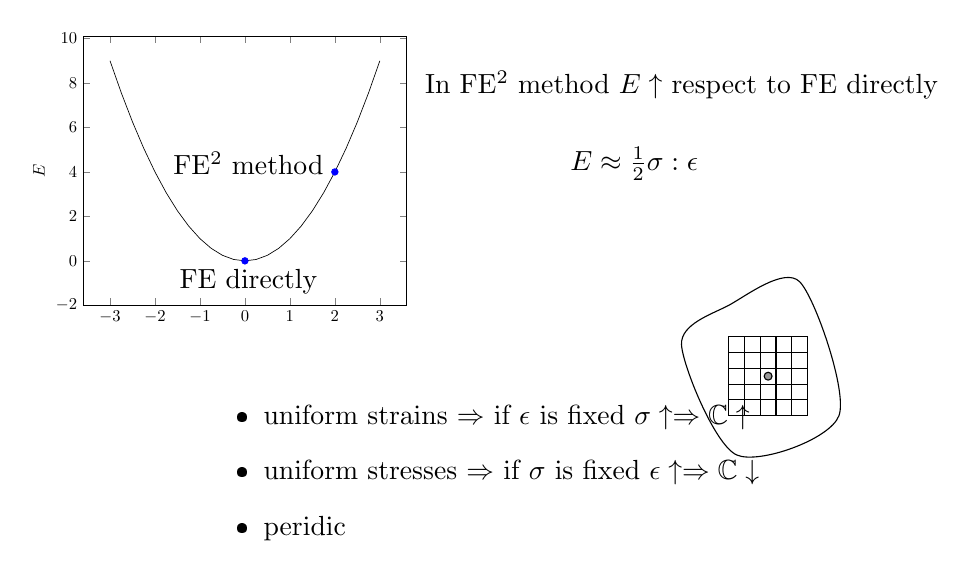
\begin{tikzpicture}
   \begin{scope}[scale=0.6, yshift=2cm]
   \begin{axis}[domain=-3:3, ylabel = $E$, ymin = -2]
    \addplot[no marks] {x^2};
    \addplot[only marks,mark=*,blue] plot coordinates {(0,0) (2,4)};
   \end{axis}
   \node at (3.5,.5) {FE directly};
   \node at (3.5,3) {FE$^2$ method};
   \end{scope}

  \node at (7.6,4) {In FE$^2$ method $E \uparrow$ respect to FE directly};
  \node at (7,3) {$E\approx\frac{1}{2}\sigma:\epsilon$};
  \node at (5,-1) {
  \begin{varwidth}{\linewidth}
  \begin{itemize}
      \item uniform strains  $\Rightarrow$ if $\epsilon$ is fixed $\sigma\uparrow \Rightarrow \mathbb{C}\uparrow$
      \item uniform stresses  $\Rightarrow$ if $\sigma$ is fixed $\epsilon\uparrow \Rightarrow \mathbb{C}\downarrow$
      \item peridic
  \end{itemize}
  \end{varwidth}
  };

  \begin{scope}[scale=0.1,xshift = 70cm,yshift = -8cm]
  \draw [black] plot [smooth cycle] coordinates {(6,15) (13,1) (26,6) (21,23) (12,20)};
  \begin{scope}[scale=1,xshift = 4cm,yshift = -2cm]
     \foreach \y [count=\n]in {8,10,12,14,16}{ 
     \foreach \x [count=\n]in {8,10,12,14,16}{ 
     \begin{scope}[yshift = \y cm,xshift = \x cm,start chain=going right]
       \draw (0,0) -- (2,0) -- (2,2) -- (0,2) -- cycle;
       %\filldraw[fill=black!40!white,draw=black] (1,1) circle (0.5cm);
     \end{scope}
     }
  }
  \filldraw[fill=black!40!white,draw=black] (13cm,13cm) circle (0.5cm);
  \end{scope}
  \end{scope}

  \end{tikzpicture}

\end{document}
}
\end{figure}
\end{frame}

%------------------------------------------------

\begin{frame}
\frametitle{The FE$^2$ multi-scale method}

\begin{figure}[!ht]
\resizebox{1.0\linewidth}{!}{\documentclass{standalone}

\begin{document}

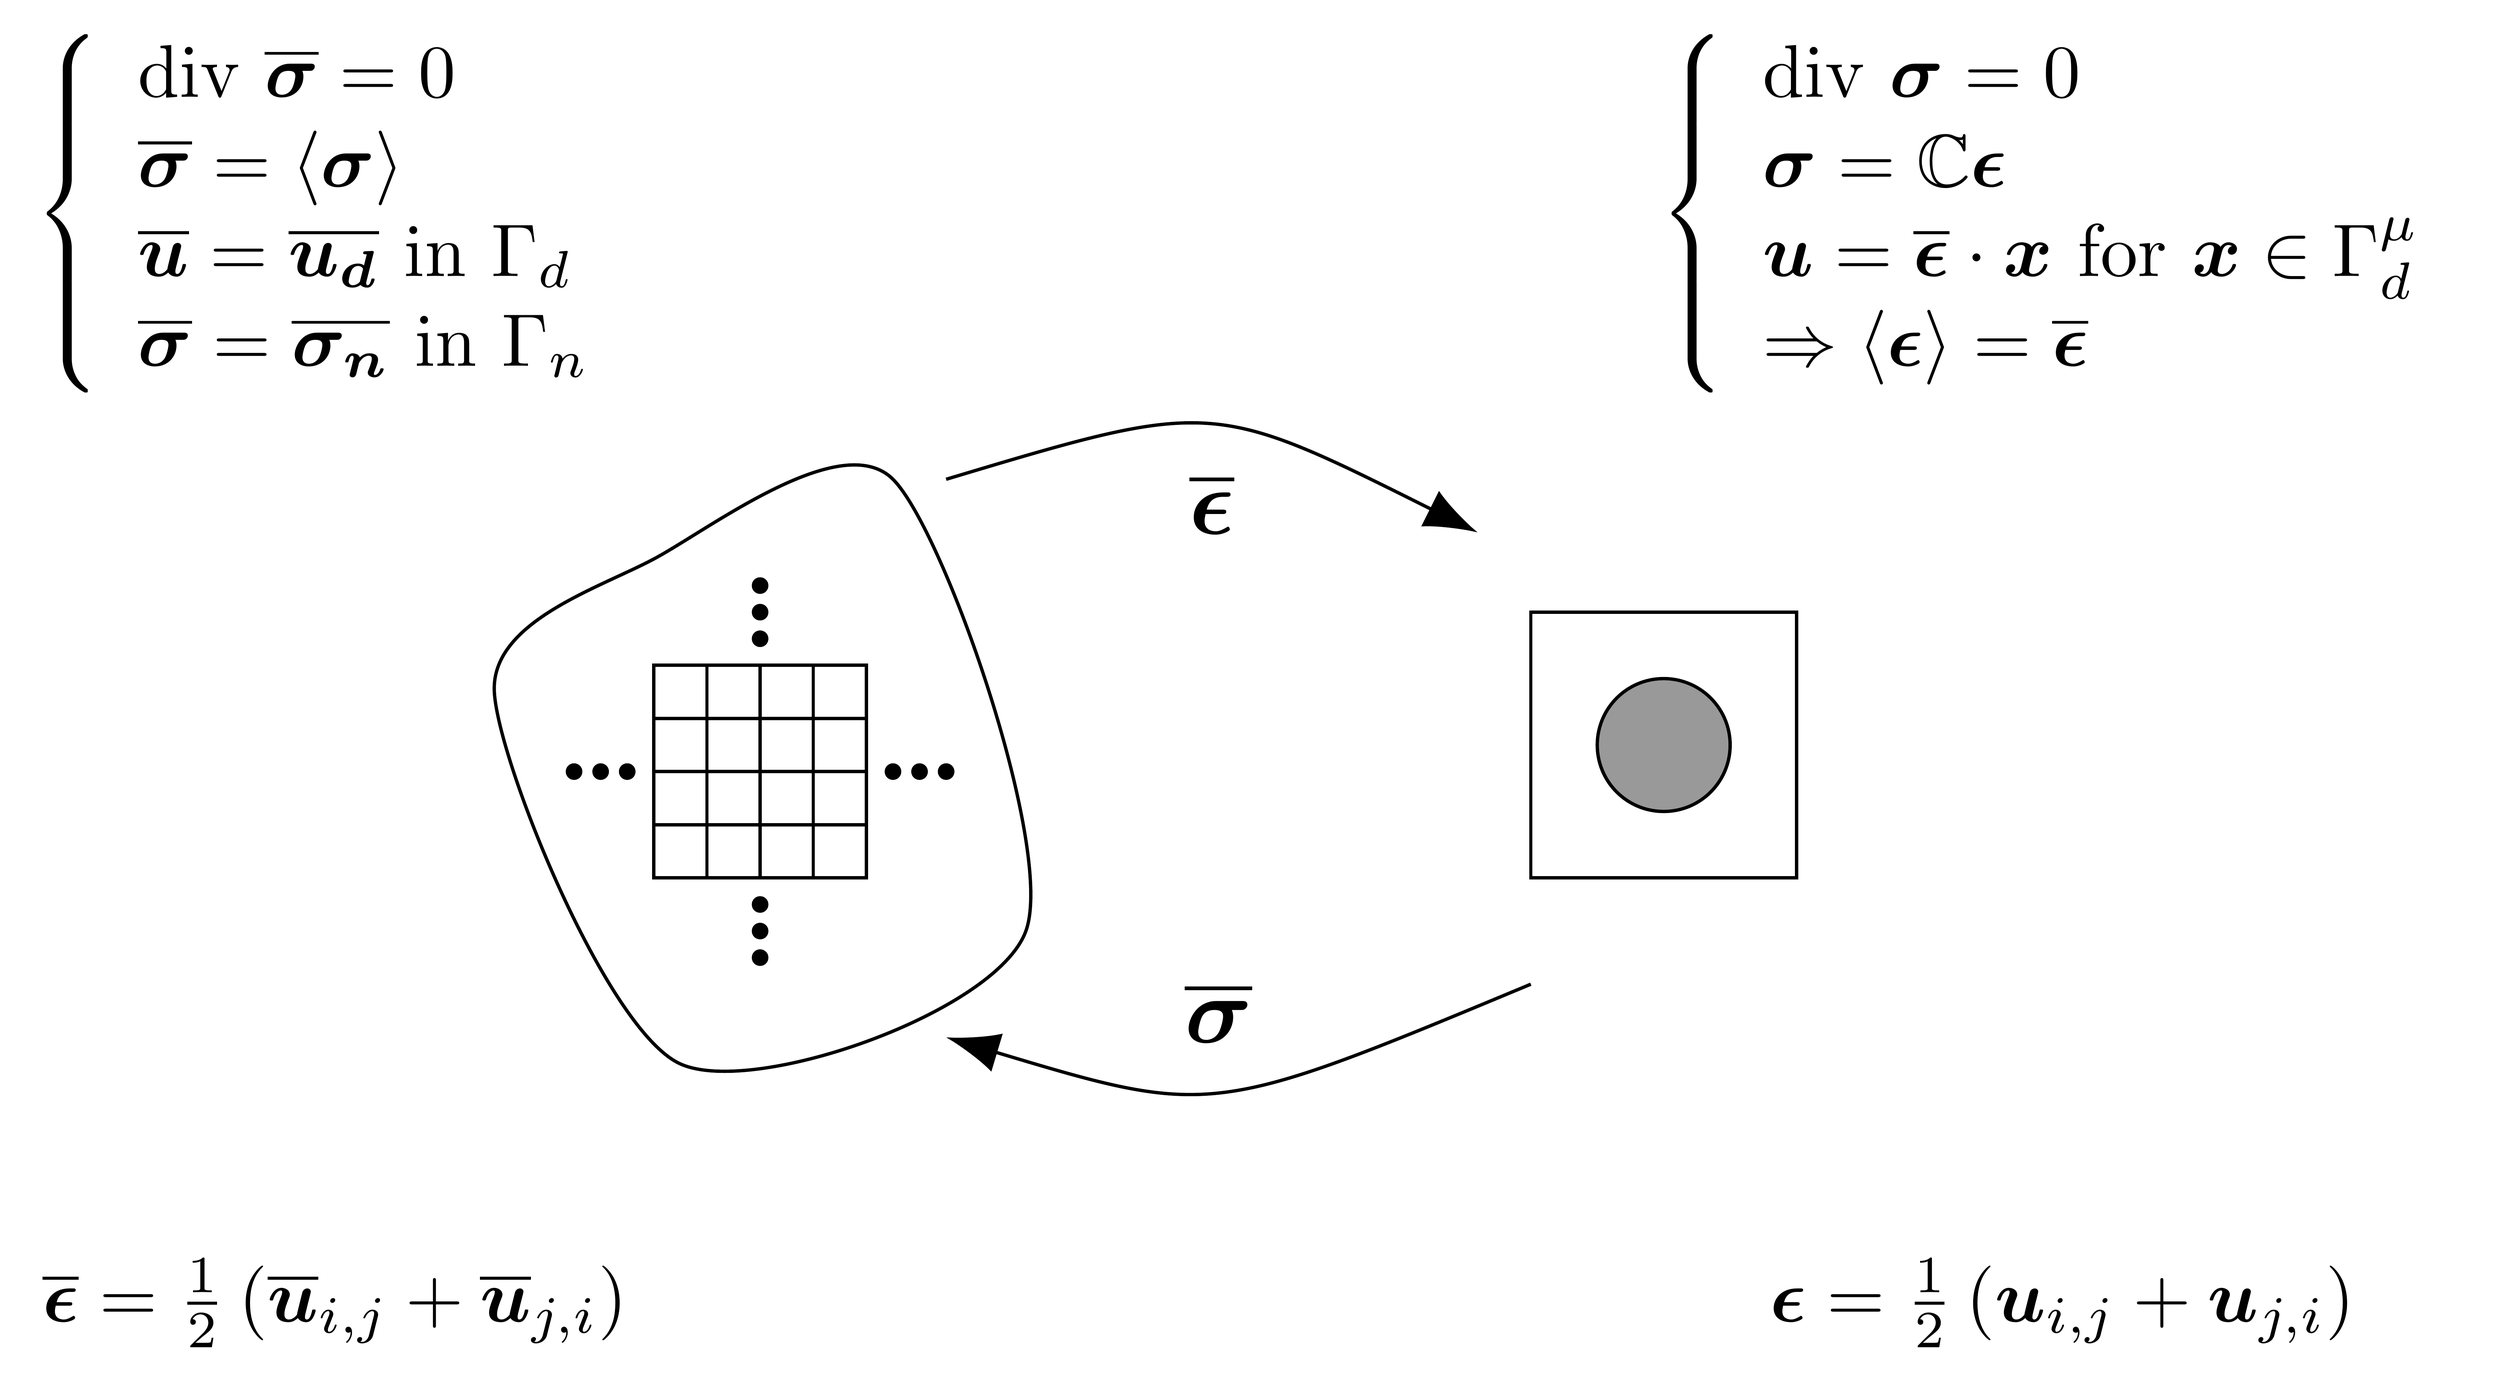
\begin{tikzpicture}[>=latex,node distance=0pt, line width=1.25mm]

% the h.m.s.

    %\draw [gray!50]  (2,0) -- (13,1) -- (26,6) -- (15,23) -- (1,20) -- cycle;
    \draw [black] plot [smooth cycle] coordinates {(6,15) (13,1) (26,6) (21,23)
    (12,20)};

    \begin{scope}[yshift = 0 cm,xshift = 4 cm]

    \foreach \y [count=\n]in {8,10,12,14}{ 
       \foreach \x [count=\n]in {8,10,12,14}{ 
         \begin{scope}[yshift = \y cm,xshift = \x cm,start chain=going right]
           \draw (0,0) -- (2,0) -- (2,2) -- (0,2) -- cycle;
           %\filldraw[fill=black!40!white,draw=black] (1,1) circle (0.5cm);
         \end{scope}
       }
    }

    \filldraw[fill=black,draw=black] (5,12) circle (0.25cm);
    \filldraw[fill=black,draw=black] (6,12) circle (0.25cm);
    \filldraw[fill=black,draw=black] (7,12) circle (0.25cm);

    \filldraw[fill=black,draw=black] (17,12) circle (0.25cm);
    \filldraw[fill=black,draw=black] (18,12) circle (0.25cm);
    \filldraw[fill=black,draw=black] (19,12) circle (0.25cm);

    \filldraw[fill=black,draw=black] (12,5) circle (0.25cm);
    \filldraw[fill=black,draw=black] (12,6) circle (0.25cm);
    \filldraw[fill=black,draw=black] (12,7) circle (0.25cm);

    \filldraw[fill=black,draw=black] (12,17) circle (0.25cm);
    \filldraw[fill=black,draw=black] (12,18) circle (0.25cm);
    \filldraw[fill=black,draw=black] (12,19) circle (0.25cm);

    \end{scope}

% the r.v.e.

    \begin{scope}[yshift = 8 cm,xshift = 45 cm,start chain=going right,scale=5]
          \draw (0,0) -- (2,0) -- (2,2) -- (0,2) -- cycle;
          \filldraw[fill=black!40!white,draw=black] (1,1) circle (0.5cm);
    \end{scope}

    \draw[-{Latex[length=20mm,width=15mm]}] (23,23) ..  controls ++(10,+3) ..
    node[below, scale=10] {$\overline{\bm{\epsilon}}$} 
    ++(20,-2);
    \draw[{Latex[length=20mm,width=15mm]}-] (23,2) .. controls ++(10,-3) .. 
    node[above, scale=10] {$\overline{\bm{\sigma}}$}
    ++(22,+2);

    \node[scale=8] at (65,33) {$
    \left\{
    \begin{array}{ll}
    \text{div } \bm{\sigma} = 0 \\
    \bm{\sigma} = \mathbb{C}\bm{\epsilon} \\
    \bm{u} = \overline{\bm{\epsilon}}\cdot \bm{x} \text{ for } \bm{x} \in \Gamma_d^\mu \\ \Rightarrow 
    \langle \bm{\epsilon} \rangle = \overline{\bm{\epsilon}}\\
    \end{array}
    \right.
    $};

    \node[scale=8] at (0,33) {$
    \left\{
    \begin{array}{ll}
    \text{div } \overline{\bm{\sigma}} = 0 \\
    \overline{\bm{\sigma}} = \langle \bm{\sigma} \rangle \\
    \overline{\bm{u}} = \overline{\bm{u_d}} \text{ in } \Gamma_d\\
    \overline{\bm{\sigma}} = \overline{\bm{\sigma_n}} \text{ in } \Gamma_n
    \end{array}
    \right.
    $};

    \node[scale=8] at (0,-8) {$\overline{\bm{\epsilon}} = \frac{1}{2} \left(\overline{\bm{u}}_{i,j} + \overline{\bm{u}}_{j,i}\right)$};
    \node[scale=8] at (65,-8) {${\bm{\epsilon}} = \frac{1}{2} \left({\bm{u}}_{i,j} + {\bm{u}}_{j,i}\right)$};

\end{tikzpicture}

\end{document}
}
\end{figure}
\end{frame}

%------------------------------------------------

\begin{frame}
\frametitle{The FE$^2$ multi-scale method}

\begin{figure}[!ht]
\resizebox{1.0\linewidth}{!}{\documentclass{standalone}

\begin{document}

\tikzset{cross/.style={cross out, draw=black, fill=none, minimum size=2*(#1-\pgflinewidth), inner sep=0pt, outer
sep=0pt}, cross/.default={2pt}}

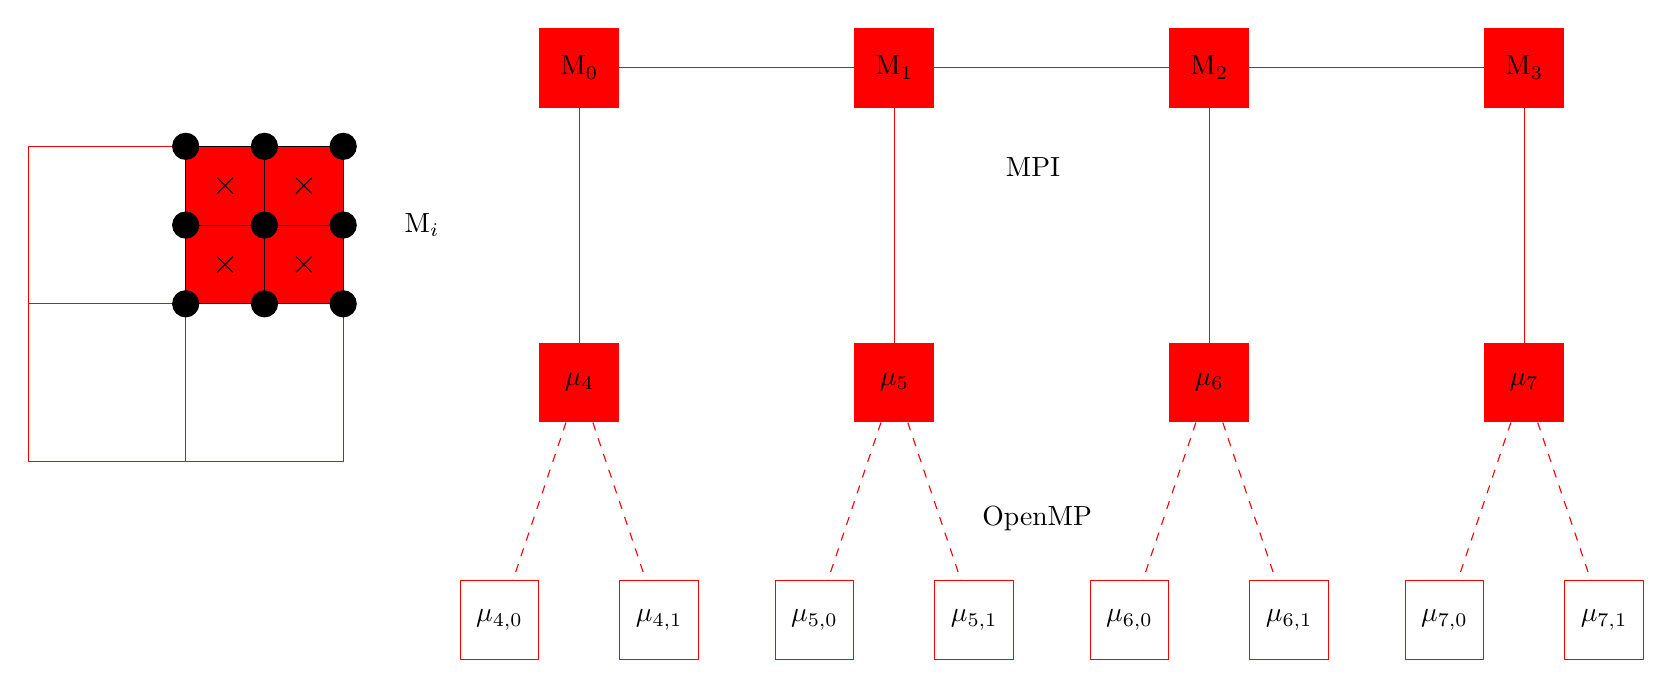
\begin{tikzpicture}[node distance=4cm]
  \tikzstyle{mpi} = [fill=red,draw=red,text=black,minimum size=1cm]
  \tikzstyle{openmp} = [fill=none,draw=red,text=black,minimum size=1cm]

  \node[mpi] (MPI_0) at (2,10) {M$_0$};
  \node[mpi] (MPI_1) [right of = MPI_0] {M$_1$};
  \node[mpi] (MPI_2) [right of = MPI_1] {M$_2$};
  \node[mpi] (MPI_3) [right of = MPI_2] {M$_3$};

  \node[mpi] (MPI_4) at (2,6) {$\mu_4$};
  \node[mpi] (MPI_5) [right of = MPI_4] {$\mu_5$};
  \node[mpi] (MPI_6) [right of = MPI_5] {$\mu_6$};
  \node[mpi] (MPI_7) [right of = MPI_6] {$\mu_7$};

  \node[openmp] (OpenMP_0) [below left = 2cm and 0cm of MPI_4] {$\mu_{4,0}$};
  \node[openmp] (OpenMP_1) [below right = 2cm and 0cm of MPI_4] {$\mu_{4,1}$};
  \node[openmp] (OpenMP_2) [below left = 2cm and 0cm of MPI_5] {$\mu_{5,0}$};
  \node[openmp] (OpenMP_3) [below right = 2cm and 0cm of MPI_5] {$\mu_{5,1}$};
  \node[openmp] (OpenMP_4) [below left = 2cm and 0cm of MPI_6] {$\mu_{6,0}$};
  \node[openmp] (OpenMP_5) [below right = 2cm and 0cm of MPI_6] {$\mu_{6,1}$};
  \node[openmp] (OpenMP_6) [below left = 2cm and 0cm of MPI_7] {$\mu_{7,0}$};
  \node[openmp] (OpenMP_7) [below right = 2cm and 0cm of MPI_7] {$\mu_{7,1}$};

  \node[draw=none,fill=none] [above right = 0.5cm and -2.5cm of OpenMP_4] {OpenMP};
  \node[draw=none,fill=none] [above right = 5.0cm and -2.2cm of OpenMP_4] {MPI};

  \draw [draw=red,-] (MPI_0) -- (MPI_1);
  \draw [draw=red,-] (MPI_1) -- (MPI_2);
  \draw [draw=red,-] (MPI_2) -- (MPI_3);

  \draw [draw=red,-] (MPI_0) -- (MPI_4);
  \draw [draw=red,-] (MPI_1) -- (MPI_5);
  \draw [draw=red,-] (MPI_2) -- (MPI_6);
  \draw [draw=red,-] (MPI_3) -- (MPI_7);

  \draw [draw=red,-,dashed] (MPI_4) -- (OpenMP_0);
  \draw [draw=red,-,dashed] (MPI_4) -- (OpenMP_1);

  \draw [draw=red,-,dashed] (MPI_5) -- (OpenMP_2);
  \draw [draw=red,-,dashed] (MPI_5) -- (OpenMP_3);

  \draw [draw=red,-,dashed] (MPI_6) -- (OpenMP_4);
  \draw [draw=red,-,dashed] (MPI_6) -- (OpenMP_5);

  \draw [draw=red,-,dashed] (MPI_7) -- (OpenMP_6);
  \draw [draw=red,-,dashed] (MPI_7) -- (OpenMP_7);

  \begin{scope}[xshift=2cm]
   \node[fill=none, draw=red, minimum size = 2cm] (square_0) at (-6,8) {};
   \node[fill=red, draw=red, minimum size = 2cm] (square_1) at (-4,8) {};
   \node[fill=none, draw=red, minimum size = 2cm] (square_2) at (-6,6) {};
   \node[fill=none, draw=red, minimum size = 2cm] (square_3) at (-4,6) {};

   \node[circle,fill=black, draw=black, minimum size = 0.05cm] (node_0) at (-5,9) {};
   \node[circle,fill=black, draw=black, minimum size = 0.05cm] (node_1) at (-4,9) {};
   \node[circle,fill=black, draw=black, minimum size = 0.05cm] (node_2) at (-3,9) {};
   \node[circle,fill=black, draw=black, minimum size = 0.05cm] (node_3) at (-5,8) {};
   \node[circle,fill=black, draw=black, minimum size = 0.05cm] (node_4) at (-4,8) {};
   \node[circle,fill=black, draw=black, minimum size = 0.05cm] (node_5) at (-3,8) {};
   \node[circle,fill=black, draw=black, minimum size = 0.05cm] (node_6) at (-5,7) {};
   \node[circle,fill=black, draw=black, minimum size = 0.05cm] (node_7) at (-4,7) {};
   \node[circle,fill=black, draw=black, minimum size = 0.05cm] (node_8) at (-3,7) {};

   \draw [draw=black,-] (-5,9) -- (-3,9);
   \draw [draw=black,-] (-5,8) -- (-3,8);
   \draw [draw=black,-] (-5,7) -- (-3,7);

   \draw [draw=black,-] (-5,9) -- (-5,7);
   \draw [draw=black,-] (-4,9) -- (-4,7);
   \draw [draw=black,-] (-3,9) -- (-3,7);

   \node[fill=none, draw=none] (title_1) at (-2,8) {M$_i$};

   \node[cross,minimum size=0.2cm] (gp_0) at (-4.5,8.5) {};
   \node[cross,minimum size=0.2cm] (gp_1) at (-3.5,8.5) {};
   \node[cross,minimum size=0.2cm] (gp_2) at (-4.5,7.5) {};
   \node[cross,minimum size=0.2cm] (gp_3) at (-3.5,7.5) {};
  \end{scope}
 \end{tikzpicture}

\end{document}
}
\end{figure}
\end{frame}

%------------------------------------------------

\begin{frame}
\begin{figure}[!ht]
\resizebox{0.8\linewidth}{!}{\documentclass{standalone}

\begin{document}

\begin{tikzpicture}[node distance=4cm]

    \node[inner sep=0pt, scale=0.1] (rve) at (0,0) {\includegraphics[width=1.4\textwidth]{figures/front_exp_0-crop.pdf}};
    \node[inner sep=0pt, scale=0.1] (rve) at (2,0) {\includegraphics[width=1.4\textwidth]{figures/front_exp_1-crop.pdf}};
    \node[inner sep=0pt, scale=0.1] (rve) at (4,0) {\includegraphics[width=1.4\textwidth]{figures/front_exp_2-crop.pdf}};
    \node[inner sep=0pt, scale=0.25] (rve) at (2,2.2) {\includegraphics[width=1.4\textwidth]{figures/prob_paper_2.pdf}};

 \end{tikzpicture}

\end{document}
}
\end{figure}
\end{frame}

%------------------------------------------------

\begin{frame}
\begin{figure}[!ht]
\resizebox{1.0\linewidth}{!}{\documentclass{standalone}

\begin{document}

\begin{tikzpicture}[node distance=4cm]

    \node[inner sep=0pt, scale=0.3] at (0,0) {\includegraphics[width=1.4\textwidth]{figures/res_paper_2.pdf}};
    \node[inner sep=0pt, scale=0.1] at (4,1) {\includegraphics[width=1.4\textwidth]{figures/fig_direct-crop.pdf}};
    \node[inner sep=0pt, scale=0.1] at (4,-1) {\includegraphics[width=1.4\textwidth]{figures/fig_homog_us-crop.pdf}};

 \end{tikzpicture}

\end{document}
}
\end{figure}
\end{frame}

%------------------------------------------------

\begin{frame}
\Huge{\centerline{The End}}
\end{frame}

%----------------------------------------------------------------------------------------

\end{document} 
